% ------------------------------------------------------------------------------
% The OpenQuake-engine Risk Quality Assurance Report
%
% Authors:
%  Anirudh Rao         - GEM Model Facility, Pavia, Italy
%
% License:
% Document distributed under the CC BY-NC-SA 4.0 License
% Creative Commons Attribution-NonCommercial-ShareAlike 4.0 International
% http://creativecommons.org/licenses/by-nc-sa/4.0/
%
% Copyright:
% © GEM Foundation, Pavia, Italy. August 2015.
%
%-------------------------------------------------------------------------------
%  PACKAGES AND OTHER DOCUMENT CONFIGURATIONS
%-------------------------------------------------------------------------------

\documentclass[11pt,fleqn]{book} % ------------------ Left-justified equations -
%%%%%%%%%%%%%%%%%%%%%%%%%%%%%%%%%%%%%%%%%
% The Legrand Orange Book
% LaTeX Template
% Version 1.4 (12/4/14)
%
% This template has been downloaded from:
% http://www.LaTeXTemplates.com
%
% Original author:
% Mathias Legrand (legrand.mathias@gmail.com)
%
% License:
% CC BY-NC-SA 3.0 (http://creativecommons.org/licenses/by-nc-sa/3.0/)
%
% Compiling this template:
% This template uses biber for its bibliography and makeindex for its index.
% When you first open the template, compile it from the command line with the 
% commands below to make sure your LaTeX distribution is configured correctly:
%
% 1) pdflatex oq-manual
% 2) makeindex oq-manual.idx -s StyleInd.ist
% 3) biber oq-manual
% 4  makeglossaries oq-manual
% 4) pdflatex oq-manual x 2
%
% After this, when you wish to update the bibliography/index use the appropriate
% command above and make sure to compile with pdflatex several times 
% afterwards to propagate your changes to the document.
%
% This template also uses a number of packages which may need to be
% updated to the newest versions for the template to compile. It is strongly
% recommended you update your LaTeX distribution if you have any
% compilation errors.
%
% Important note:
% Chapter heading images should have a 2:1 width:height ratio,
% e.g. 920px width and 460px height.
%
%%%%%%%%%%%%%%%%%%%%%%%%%%%%%%%%%%%%%%%%%
\linespread{1.2} % Increase default line spacing
\usepackage[top=3cm,bottom=3cm,left=3.2cm,right=3.2cm,headsep=10pt,a4paper]{geometry} % Page margins

\usepackage{xcolor} % Required for specifying colors by name
\definecolor{ocre}{RGB}{243,102,25} % Define the orange color used for highlighting throughout the book

% Font Settings
\usepackage{avant} % Use the Avantgarde font for headings
%\usepackage{times} % Use the Times font for headings
\usepackage{mathptmx} % Use the Adobe Times Roman as the default text font together with math symbols from the Sym­bol, Chancery and Com­puter Modern fonts

\usepackage{microtype} % Slightly tweak font spacing for aesthetics
\usepackage[utf8]{inputenc} % Required for including letters with accents
\usepackage[T1]{fontenc} % Use 8-bit encoding that has 256 glyphs

% Bibliography
\usepackage{csquotes}
\usepackage[style=alphabetic,
            sorting=nyt,
            sortcites=true,
            natbib=true,
            style=authoryear,
            maxcitenames=2,
            maxbibnames=100,
            autopunct=true,
            autolang=hyphen,
            hyperref=true,
            doi=true,
            abbreviate=false,
            backref=true,
            backend=bibtex,
	    	uniquename=false,
	    	uniquelist=false]{biblatex}
\addbibresource{bibliography/qa.bib}
\defbibheading{bibempty}{}

% Figure caption settings
\usepackage[textfont=it,margin=10pt,font=small,labelfont=bf,labelsep=endash]{caption}
\usepackage{subcaption}
\usepackage{rotating}

% Table - colors from
\usepackage{verbatim}
\usepackage{fancyvrb}
\usepackage{color, colortbl}
\definecolor{darkgray}{gray}{0.25}
\definecolor{darkblue}{rgb}{.2, .2, .8}
\definecolor{almond}{rgb}{0.94, 0.87, 0.8}
\definecolor{ashgrey}{rgb}{0.7, 0.75, 0.71}
\definecolor{anti-flashwhite}{rgb}{0.95, 0.95, 0.96}
\definecolor{anti-flashwhite}{rgb}{0.95, 0.95, 0.96}
\definecolor{airforceblue}{rgb}{0.36, 0.54, 0.66}

% Index
\usepackage{calc} % For simpler calculation - used for spacing the index letter headings correctly
\usepackage{makeidx} % Required to make an index
\setcounter{secnumdepth}{3}
\setcounter{tocdepth}{3}    % entries down to \subsubsections in the TOC
\makeindex % Tells LaTeX to create the files required for indexing

\usepackage{todonotes}
\usepackage{marginnote}

% package for bold symbols
\usepackage{bm}

% for better looking tables
\usepackage{ctable}
%
%----------------------------------------------------------------------------------------
% Trees
% \usepackage{auto-pst-pdf}
% \usepackage[pdf]{pstricks}
% \usepackage{pst-tree} % -------------------- Load packages -
%----------------------------------------------------------------------------------------
%	VARIOUS REQUIRED PACKAGES
%----------------------------------------------------------------------------------------

\usepackage{titlesec} % Allows customization of titles

\usepackage{graphicx} % Required for including pictures
\graphicspath{{figures/}} % Specifies the directory where pictures are stored

\usepackage{tikz} % Required for drawing custom shapes

\usepackage[english]{babel} % English language/hyphenation

\usepackage{enumitem} % Customize lists
\setlist{nolistsep} % Reduce spacing between bullet points and numbered lists

\usepackage{booktabs} % Required for nicer horizontal rules in tables

\usepackage{eso-pic} % Required for specifying an image background in the title page

\usepackage{pdfpages} % Needed to load .pdf pages

%----------------------------------------------------------------------------------------
%	MAIN TABLE OF CONTENTS
%----------------------------------------------------------------------------------------

\usepackage{titletoc} % Required for manipulating the table of contents

\contentsmargin{0cm} % Removes the default margin
% Chapter text styling
\titlecontents{chapter}[1.25cm] % Indentation
{\addvspace{15pt}\large\sffamily\bfseries} % Spacing and font options for chapters
{\color{ocre!60}\contentslabel[\Large\thecontentslabel]{1.25cm}\color{ocre}} % Chapter number
{}  
{\color{ocre!60}\normalsize\sffamily\bfseries\;\titlerule*[.5pc]{.}\;\thecontentspage} % Page number
% Section text styling
\titlecontents{section}[1.25cm] % Indentation
{\addvspace{5pt}\sffamily\bfseries} % Spacing and font options for sections
{\contentslabel[\thecontentslabel]{1.25cm}} % Section number
{}
{\sffamily\hfill\color{black}\thecontentspage} % Page number
[]
% Subsection text styling
\titlecontents{subsection}[1.25cm] % Indentation
{\addvspace{1pt}\sffamily\small} % Spacing and font options for subsections
{\contentslabel[\thecontentslabel]{1.25cm}} % Subsection number
{}
{\sffamily\;\titlerule*[.5pc]{.}\;\thecontentspage} % Page number
[] 

%----------------------------------------------------------------------------------------
%	MINI TABLE OF CONTENTS IN CHAPTER HEADS
%----------------------------------------------------------------------------------------

% Section text styling
\titlecontents{lsection}[0em] % Indendating
{\footnotesize\sffamily} % Font settings
{}
{}
{}

% Subsection text styling
\titlecontents{lsubsection}[.5em] % Indentation
{\normalfont\footnotesize\sffamily} % Font settings
{}
{}
{}
 
%----------------------------------------------------------------------------------------
%	PAGE HEADERS
%----------------------------------------------------------------------------------------

\usepackage{fancyhdr} % Required for header and footer configuration

\pagestyle{fancy}
\renewcommand{\chaptermark}[1]{\markboth{\sffamily\normalsize\bfseries\chaptername\ \thechapter.\ #1}{}} % Chapter text font settings
\renewcommand{\sectionmark}[1]{\markright{\sffamily\normalsize\thesection\hspace{5pt}#1}{}} % Section text font settings
\fancyhf{} \fancyhead[LE,RO]{\sffamily\normalsize\thepage} % Font setting for the page number in the header
\fancyhead[LO]{\rightmark} % Print the nearest section name on the left side of odd pages
\fancyhead[RE]{\leftmark} % Print the current chapter name on the right side of even pages
\renewcommand{\headrulewidth}{0.5pt} % Width of the rule under the header
\addtolength{\headheight}{2.5pt} % Increase the spacing around the header slightly
\renewcommand{\footrulewidth}{0pt} % Removes the rule in the footer
\fancypagestyle{plain}{\fancyhead{}\renewcommand{\headrulewidth}{0pt}} % Style for when a plain pagestyle is specified

% Removes the header from odd empty pages at the end of chapters
\makeatletter
\renewcommand{\cleardoublepage}{
\clearpage\ifodd\c@page\else
\hbox{}
\vspace*{\fill}
\thispagestyle{empty}
\newpage
\fi}

%----------------------------------------------------------------------------------------
%	THEOREM STYLES
%----------------------------------------------------------------------------------------

\usepackage{amsmath,amsfonts,amssymb,amsthm} % For math equations, theorems, symbols, etc

\newcommand{\intoo}[2]{\mathopen{]}#1\,;#2\mathclose{[}}
\newcommand{\ud}{\mathop{\mathrm{{}d}}\mathopen{}}
\newcommand{\intff}[2]{\mathopen{[}#1\,;#2\mathclose{]}}
\newtheorem{notation}{Notation}[chapter]

%%%%%%%%%%%%%%%%%%%%%%%%%%%%%%%%%%%%%%%%%%%%%%%%%%%%%%%%%%%%%%%%%%%%%%%%%%%
%%%%%%%%%%%%%%%%%%%% dedicated to boxed/framed environements %%%%%%%%%%%%%%
%%%%%%%%%%%%%%%%%%%%%%%%%%%%%%%%%%%%%%%%%%%%%%%%%%%%%%%%%%%%%%%%%%%%%%%%%%%
\newtheoremstyle{ocrenumbox}% % Theorem style name
{0pt}% Space above
{0pt}% Space below
{\normalfont}% % Body font
{}% Indent amount
{\small\bf\sffamily\color{ocre}}% % Theorem head font
{\;}% Punctuation after theorem head
{0.25em}% Space after theorem head
{\small\sffamily\color{ocre}\thmname{#1}\nobreakspace\thmnumber{\@ifnotempty{#1}{}\@upn{#2}}% Theorem text (e.g. Theorem 2.1)
\thmnote{\nobreakspace\the\thm@notefont\sffamily\bfseries\color{black}---\nobreakspace#3.}} % Optional theorem note
\renewcommand{\qedsymbol}{$\blacksquare$}% Optional qed square

\newtheoremstyle{blacknumex}% Theorem style name
{5pt}% Space above
{5pt}% Space below
{\normalfont}% Body font
{} % Indent amount
{\small\bf\sffamily}% Theorem head font
{\;}% Punctuation after theorem head
{0.25em}% Space after theorem head
{\small\sffamily{\tiny\ensuremath{\blacksquare}}\nobreakspace\thmname{#1}\nobreakspace\thmnumber{\@ifnotempty{#1}{}\@upn{#2}}% Theorem text (e.g. Theorem 2.1)
\thmnote{\nobreakspace\the\thm@notefont\sffamily\bfseries---\nobreakspace#3.}}% Optional theorem note

\newtheoremstyle{blacknumbox} % Theorem style name
{0pt}% Space above
{0pt}% Space below
{\normalfont}% Body font
{}% Indent amount
{\small\bf\sffamily}% Theorem head font
{\;}% Punctuation after theorem head
{0.25em}% Space after theorem head
{\small\sffamily\thmname{#1}\nobreakspace\thmnumber{\@ifnotempty{#1}{}\@upn{#2}}% Theorem text (e.g. Theorem 2.1)
\thmnote{\nobreakspace\the\thm@notefont\sffamily\bfseries---\nobreakspace#3.}}% Optional theorem note

%%%%%%%%%%%%%%%%%%%%%%%%%%%%%%%%%%%%%%%%%%%%%%%%%%%%%%%%%%%%%%%%%%%%%%%%%%%
%%%%%%%%%%%%% dedicated to non-boxed/non-framed environements %%%%%%%%%%%%%
%%%%%%%%%%%%%%%%%%%%%%%%%%%%%%%%%%%%%%%%%%%%%%%%%%%%%%%%%%%%%%%%%%%%%%%%%%%
\newtheoremstyle{ocrenum}% % Theorem style name
{5pt}% Space above
{5pt}% Space below
{\normalfont}% % Body font
{}% Indent amount
{\small\bf\sffamily\color{ocre}}% % Theorem head font
{\;}% Punctuation after theorem head
{0.25em}% Space after theorem head
{\small\sffamily\color{ocre}\thmname{#1}\nobreakspace\thmnumber{\@ifnotempty{#1}{}\@upn{#2}}% Theorem text (e.g. Theorem 2.1)
\thmnote{\nobreakspace\the\thm@notefont\sffamily\bfseries\color{black}---\nobreakspace#3.}} % Optional theorem note
\renewcommand{\qedsymbol}{$\blacksquare$}% Optional qed square
\makeatother

% Defines the theorem text style for each type of theorem to one of the three styles above
\newcounter{dummy} 
\numberwithin{dummy}{section}
\theoremstyle{ocrenumbox}
\newtheorem{theoremeT}[dummy]{Theorem}
\newtheorem{problem}{Problem}[chapter]
\newtheorem{exerciseT}{Exercise}[chapter]
\theoremstyle{blacknumex}
\newtheorem{exampleT}{Example}[chapter]
\theoremstyle{blacknumbox}
\newtheorem{vocabulary}{Vocabulary}[chapter]
\newtheorem{definitionT}{Definition}[section]
\newtheorem{corollaryT}[dummy]{Corollary}
\theoremstyle{ocrenum}
\newtheorem{proposition}[dummy]{Proposition}

%----------------------------------------------------------------------------------------
%	DEFINITION OF COLORED BOXES
%----------------------------------------------------------------------------------------

\RequirePackage[framemethod=default]{mdframed} % Required for creating the theorem, definition, exercise and corollary boxes

% Theorem box
\newmdenv[skipabove=7pt,
skipbelow=7pt,
backgroundcolor=black!5,
linecolor=ocre,
innerleftmargin=5pt,
innerrightmargin=5pt,
innertopmargin=5pt,
leftmargin=0cm,
rightmargin=0cm,
innerbottommargin=5pt]{tBox}

% Exercise box	  
\newmdenv[skipabove=7pt,
skipbelow=7pt,
rightline=false,
leftline=true,
topline=false,
bottomline=false,
backgroundcolor=ocre!10,
linecolor=ocre,
innerleftmargin=5pt,
innerrightmargin=5pt,
innertopmargin=5pt,
innerbottommargin=5pt,
leftmargin=0cm,
rightmargin=0cm,
linewidth=4pt]{eBox}	

% Definition box
\newmdenv[skipabove=7pt,
skipbelow=7pt,
rightline=false,
leftline=true,
topline=false,
bottomline=false,
linecolor=ocre,
innerleftmargin=5pt,
innerrightmargin=5pt,
innertopmargin=0pt,
leftmargin=0cm,
rightmargin=0cm,
linewidth=4pt,
innerbottommargin=0pt]{dBox}	

% Corollary box
\newmdenv[skipabove=7pt,
skipbelow=7pt,
rightline=false,
leftline=true,
topline=false,
bottomline=false,
linecolor=gray,
backgroundcolor=black!5,
innerleftmargin=5pt,
innerrightmargin=5pt,
innertopmargin=5pt,
leftmargin=0cm,
rightmargin=0cm,
linewidth=4pt,
innerbottommargin=5pt]{cBox}

% Creates an environment for each type of theorem and assigns it a theorem text style from the "Theorem Styles" section above and a colored box from above
\newenvironment{theorem}{\begin{tBox}\begin{theoremeT}}{\end{theoremeT}\end{tBox}}
\newenvironment{exercise}{\begin{eBox}\begin{exerciseT}}{\hfill{\color{ocre}\tiny\ensuremath{\blacksquare}}\end{exerciseT}\end{eBox}}				  
\newenvironment{definition}{\begin{dBox}\begin{definitionT}}{\end{definitionT}\end{dBox}}	
\newenvironment{example}{\begin{exampleT}}{\hfill{\tiny\ensuremath{\blacksquare}}\end{exampleT}}		
\newenvironment{corollary}{\begin{cBox}\begin{corollaryT}}{\end{corollaryT}\end{cBox}}	

%----------------------------------------------------------------------------------------
%	REMARK ENVIRONMENT
%----------------------------------------------------------------------------------------

\newenvironment{remark}{\par\vspace{10pt}\small % Vertical white space above the remark and smaller font size
\begin{list}{}{
\leftmargin=35pt % Indentation on the left
\rightmargin=25pt}\item\ignorespaces % Indentation on the right
\makebox[-2.5pt]{\begin{tikzpicture}[overlay]
\node[draw=ocre!60,line width=1pt,circle,fill=ocre!25,font=\sffamily\bfseries,inner sep=2pt,outer sep=0pt] at (-15pt,0pt){\textcolor{ocre}{R}};\end{tikzpicture}} % Orange R in a circle
\advance\baselineskip -1pt}{\end{list}\vskip5pt} % Tighter line spacing and white space after remark

%----------------------------------------------------------------------------------------
%	SECTION NUMBERING IN THE MARGIN
%----------------------------------------------------------------------------------------

\makeatletter
\renewcommand{\@seccntformat}[1]{\llap{\textcolor{ocre}{\csname the#1\endcsname}\hspace{1em}}}                    
\renewcommand{\section}{\@startsection{section}{1}{\z@}
{-4ex \@plus -1ex \@minus -.4ex}
{1ex \@plus.2ex }
{\normalfont\large\sffamily\bfseries}}
\renewcommand{\subsection}{\@startsection {subsection}{2}{\z@}
{-3ex \@plus -0.1ex \@minus -.4ex}
{0.5ex \@plus.2ex }
{\normalfont\sffamily\bfseries}}
\renewcommand{\subsubsection}{\@startsection {subsubsection}{3}{\z@}
{-2ex \@plus -0.1ex \@minus -.2ex}
{.2ex \@plus.2ex }
{\normalfont\small\sffamily\bfseries}}                        
\renewcommand\paragraph{\@startsection{paragraph}{4}{\z@}
{-2ex \@plus-.2ex \@minus .2ex}
{.1ex}
{\normalfont\small\sffamily\bfseries}}

%----------------------------------------------------------------------------------------
%	HYPERLINKS IN THE DOCUMENTS
%----------------------------------------------------------------------------------------

% For an unclear reason, the package should be loaded now and not later
\usepackage{hyperref}
\hypersetup{hidelinks,backref=true,pagebackref=true,hyperindex=true,colorlinks=false,breaklinks=true,urlcolor= ocre,bookmarks=true,bookmarksopen=false,pdftitle={Title},pdfauthor={Author}}

%----------------------------------------------------------------------------------------
%	CHAPTER HEADINGS
%----------------------------------------------------------------------------------------

% The set-up below should be (sadly) manually adapted to the overall margin page
% septup controlled by the geometry package loaded in the main.tex document. It
% is possible to implement below the dimensions used in the goemetry package
% (top,bottom,left,right)... TO BE DONE

\newcommand{\thechapterimage}{}
\newcommand{\chapterimage}[1]{\renewcommand{\thechapterimage}{#1}}

% Numbered chapters with mini tableofcontents
\def\thechapter{\arabic{chapter}}
\def\@makechapterhead#1{
\thispagestyle{empty}
{\centering \normalfont\sffamily
\ifnum \c@secnumdepth >\m@ne
\if@mainmatter
\startcontents
\begin{tikzpicture}[remember picture,overlay]
\node at (current page.north west)
{\begin{tikzpicture}[remember picture,overlay]
\node[anchor=north west,inner sep=0pt] at (0,0) {\includegraphics[width=\paperwidth]{\thechapterimage}};
%%%%%%%%%%%%%%%%%%%%%%%%%%%%%%%%%%%%%%%%%%%%%%%%%%%%%%%%%%%%%%%%%%%%%%%%%%%%%%%%%%%%%
% Commenting the 3 lines below removes the small contents box in the chapter heading
\fill[color=ocre!10!white,opacity=.6] (1cm,0) rectangle (8cm,-7cm);
\node[anchor=north west] at (1.1cm,.35cm) {\parbox[t][8cm][t]{6.5cm}{
    \huge\bfseries\flushleft \printcontents{l}{1}{\setcounter{tocdepth}{2}}}};
\draw[anchor=west] (5cm,-9cm) node [rounded corners=20pt,fill=ocre!10!white,text opacity=1,draw=ocre,draw opacity=1,line width=1.5pt,fill opacity=.6,inner sep=12pt]{\huge\sffamily\bfseries\textcolor{black}{\thechapter. #1\strut\makebox[22cm]{}}};
%%%%%%%%%%%%%%%%%%%%%%%%%%%%%%%%%%%%%%%%%%%%%%%%%%%%%%%%%%%%%%%%%%%%%%%%%%%%%%%%%%%%%
\end{tikzpicture}};
\end{tikzpicture}}
\par\vspace*{230\p@}
\fi
\fi}

% Unnumbered chapters without mini tableofcontents (could be added though) 
\def\@makeschapterhead#1{
\thispagestyle{empty}
{\centering \normalfont\sffamily
\ifnum \c@secnumdepth >\m@ne
\if@mainmatter
\begin{tikzpicture}[remember picture,overlay]
\node at (current page.north west)
{\begin{tikzpicture}[remember picture,overlay]
\node[anchor=north west,inner sep=0pt] at (0,0) {\includegraphics[width=\paperwidth]{\thechapterimage}};
\draw[anchor=west] (5cm,-9cm) node [rounded corners=20pt,fill=ocre!10!white,fill opacity=.6,inner sep=12pt,text opacity=1,draw=ocre,draw opacity=1,line width=1.5pt]{\huge\sffamily\bfseries\textcolor{black}{#1\strut\makebox[22cm]{}}};
\end{tikzpicture}};
\end{tikzpicture}}
\par\vspace*{230\p@}
\fi
\fi
}
\makeatother
 % ------------------------ Load template -

\begin{document}
% OpenQuake Book Glossary
% To cite a glossary element in a document:
%	\gls{seismicsourcedata}
%	\Gls{seismicsourcedata} - First initial is uppercase
%	\GLS{seismicsourcedata} - All initials are uppercase
%	\glspl{seismicsourcedata} - Plural
% To process the glossary:
% 	makeglossaries oqb

%
% ------- A
\newglossaryentry{areasource}{
	name = area source,
	description={A source type usually adopted to model distributed 
	seismicity. In an area source the seismicity occurrence rate 
    is assumed uniform over the source area; this produces an hazard 
    pattern with a plateau of constant hazard inside the polygon 
    delimiting the area source and values of hazard that tend to 
    decrease as we move away from the border of the source}
}
\newglossaryentry{asset}{
    name = asset,
    description={An asset is an element with a certain value, which can include buildings or population. For example, an asset can include an individual building at a given location, or a number of buildings that are grouped, co-located at a single location and classified with the same \gls{taxonomy}}.
}
%
% ------- B
\newglossaryentry{branch}{
	name = branch,
	plural= branches,
	description={
	The simplest element in a logic tree; it belongs to a 
	\gls{branchset} where it represents one possible option among a finite 
	number of alternatives. A branch is associated with a weight 
	value \citep{scherbaum2011} if the \gls{branchset} represents the 
	epistemic uncertainty on a parameter or a model when the \gls{branchset} 
	is used to specify alternative models (e.g. district \glspl{acr:mfd})
	}
}
\newglossaryentry{branchinglevel}{
	name = branching level,
	description={It indicates the position where a \gls{branchset} or a 
	\gls{branch} is located in a logic tree structure. For example, 
	the first branching level of the 
	\gls{seismicsourcelogictree} always contains one or several 
	\glspl{initialseismicsourceinputmodel}
	}
}
\newglossaryentry{branchset}{
	name = branch set,
	description={The structure describing the epistemic uncertainty on 
	a specific parameter or model included in a logic tree structure. 
	It ensembles a number of \glspl{branch}, each one representing a 
	discrete alternative}
}
%
% ------- C
\newacronym{cpsha}{cPSHA}{Classical PSHA}
\newglossaryentry{configurationfile}{
	name =  configuration file,
	description = {
	Usually the file containing the information necessary to run a calculation
	in OpenQuake
	}
}
\newglossaryentry{charfaultsource}{
	name = characteristic fault source,
	description={
	A fault source typology where ruptures always cover the entire fault surface
	}
}
\newglossaryentry{complexfaultsource}{
	name = complex fault source,
	description={
	A source typology usually adopted to model subduction interface faults
	}
}
%
% ------- D

\newglossaryentry{deductible}{
	name = deductible,
	description = {A parameter used in the calculation of insured losses that establishes the economic value that needs to be deducted from the ground-up losses.}
}

\newglossaryentry{seismichazarddisaggregation}{
	name =  seismic hazard disaggregation,
	description = {
	A methodology to investigate the contributions to a specific
	level of hazard in terms of fundamental variables commonly used
	to characterize seismic sources and ground motion models (e.g. 
	magnitude, source-site distance, \gls{epsilon}}
}
\newglossaryentry{dip}{
	name = dip,
	description={
    The dip is the steepest angle of descent of the fault plane
    relative to a horizontal plane; it is measured in degrees [0,90] 
	}
}
\newglossaryentry{disaggregationmatrix}{
	name =  disaggregation matrix,
	description = {
	A multi-dimensional matrix used to systematically store the contributions
	to a level of hazard to be disaggregated and that is specified by the 
	user.
	See also \gls{seismichazarddisaggregation}}
}
%
% ------- E
\newacronym{acr:erf}{ERF}{Earthquake\- Rup\-ture\- Forecast}
\newacronym{acr:epsha}{ePSHA}{Event-based PSHA}
%
\newglossaryentry{earthquakeruptureforecast}{
	name = earthquake rupture forecast,
	description={
	A list of all possible ruptures generated by all the sources included 
	in a seismic source model. Each element in the list contains: the rupture 
	geometry and the rupture probability of occurrence in a given time span. 
	%
	See also the definition available on the 
	\href{http://www.opensha.org/glossary-earthquakeRuptureForecast}
	{OpenSHA website}}
}
\newglossaryentry{earthquakeruptureforecastcalculator}{
	name = earthquake rupture forecast calculator,
	description={
	Calculator producing a \gls{seismicsourcemodel} from a 
	\gls{seismicsourcelogictree} 
	}
}
%
\newglossaryentry{epsilon}{
	name = epsilon,
	description={
	normalized residual of the ground motion}
}
%
\newglossaryentry{epsha}{
	name = event-based seismic hazard analysis,
	description={
        Calculation of seismic hazard through a Monte Carlo based procedure.
	}
}
\newglossaryentry{exposure model}{
	name = exposure model,
	description={
	A set of \glspl{asset} grouped according to their geographical location, 
	\gls{taxonomy} and value}
}
%
% ------- F
\newglossaryentry{faulttrace}{
	name = fault trace,
	description={A curve representing the intersection between the surface 
    containing the fault surface (or its prolongation) 
	and the topographic surface.
    \begin{figure}[!ht]
    \centering
    \includegraphics[width=10cm]{./figures/hazard/single_rupture.pdf}
    \end{figure}
    }
}
\newglossaryentry{fragility function}{
	name = fragility function,
	description = {the probability of exceeding a set of limit states, 
	given an intensity measure level. These functions can be discrete or
	continuous}
}
\newglossaryentry{fragility model}{
	name = fragility model,
	description = {A set of \glspl{fragility function} used to model the 
	fragility of all the \glspl{asset} in the \gls{exposure model}.}
}
\newglossaryentry{frequencymagnitudedistribution}{
	name = magnitude-frequency distribution,
	description = {See \gls{mfd}
	}
}
%
% ------- G
\newacronym{acr:gem}{GEM}{Global Earthquake Model}
\newacronym{acr:gmf}{GMF}{Ground Motion Field}
\newacronym{acr:gmpe}{GMPE}{Ground Motion Prediction Equation}
\newacronym{acr:gsim}{GSIM}{Ground Shaking Intensity Model}
\newacronym{acr:gmm}{GMM}{Ground Motion Model}
\newacronym{acr:gmlt}{GMLT}{Ground Motion Logic Tree (see 
    \gls{groundmotionlogictree}}

\newglossaryentry{gridsource}{
	name = grid source,
	description={
	It's a source typology usually adopted to model distributed 
	seismicity. It's routinely produced by a seismicity smoothing 
	algorithm (one of the most famous algorithm is the one proposed 
	by \citet{frankel1995})}
}
\newglossaryentry{groundmotionfield}{
	name = ground-motion field,
	description={An object describing the geographic distribution around 
	a rupture of a ground motion intensity measure}
}
\newglossaryentry{groundmotionfieldcalc}{
	name = ground-motion field calculator,
	description={An \gls{acr:oqe} calculator that given a rupture computes the 
	geographic distribution of a ground motion intensity parameter. Currently
	OQ can generate ground motion fields using a \gls{acr:gmpe}}
}
\newglossaryentry{groundmotionlogictree}{
	name = ground-motion logic tree,
	description={A method used to systematically describe the epistemic 
	uncertainties related to the ground motion models used in the 
	computation of hazard using a specific \gls{pshainputmodel}}
}
\newglossaryentry{groundmotionmodel}{
	name = ground-motion model,
	description={An object that given a rupture with specific properties
	computes the expected ground motion at the given site. In simplest case 
	a ground motion model corresponds to a \gls{groundmotionpredictioneq}. 
	In case of complex PSHA input models, the produced ground motion models 
	contains a set of \glspl{acr:gmpe}, one for each tectonic region considered.
	}
}
\newglossaryentry{groundmotionparameter}{
	name = ground-motion parameter,
	description={A scalar or vector quantity describing a relevant property
	    of the shaking such as intensity (e.g. PGA or Spectral Acceleration) 
	    or duration, equivalent number of cycles 
	    \citep[see for example][]{hancock2005})
	}
}
\newglossaryentry{groundmotionpredictioneq}{
	name = ground-motion prediction equation,
	description={
		An equation that - given some fundamental parameters characterizing 
		the source, the propagation path and the site (in the simplest 
		case magnitude, distance and V$_\text{S,30}$) - computes the 
		value $GM$ of a (scalar) ground motion intensity parameter.
	}
}
\newglossaryentry{groundmotionsystem}{
	name = ground-motion system,
	description={An object containing a list of \gls{groundmotionlogictree}}
}
%
% ------- I 
\newglossaryentry{initialseismicsourceinputmodel}{
	name = initial seismic source input model,
	description={It's the ensable of information needed to fully describe 
        the seismic sources composing a seismic source input model. The 
        initial seismic source input model is included in the first 
	    branching level of a seismic source logic tree}
}
\newacronym{acr:imt}{IMT}{Intensity Measure Type}
\newglossaryentry{initialseismicsourcemodel}{
	name = initial seismic source model,
	description={It's a \gls{seismicsourcemodel} included in the first 
	branching level of a seismic source logic tree}
}
\newglossaryentry{insured losses}{
	name = insured losses,
	description = {Fraction of the ground-up losses that can be covered by the insurance industry, according to a certain policy.}
}

\newglossaryentry{investigationtime}{
	name = investigation time,
	description={The time interval considered to calculate hazard; usually 
	it corresponds to 50 years}
}
%
% ------- L
\newglossaryentry{limit}{
	name = limit,
	description = {A parameter used in the calculation of insured losses that establishes the maximum economic amount that can be covered by the insurance industry, according to a certain insurance policy.}
}
\newglossaryentry{logictree}{
	name = logic tree,
	description={Data structure used to systematically describe uncertainties
	on parameters and models used in a PSHA study}
}
\newglossaryentry{logictreeprocessor}{
	name = logic tree processor,
	description={An OQ calculator that takes the PSHA Input Model and creates 
	many realisations of a \gls{seismicsourcemodel} and of a 
	\gls{groundmotionmodel}}
} 
\newacronym{acr:ltmcs}{LTMCS}{Logic Tree Monte Carlo Sampler}
%
%
\newacronym{acr:msr}{MSR}{Magnitude-Scaling Relationship}
\newglossaryentry{msr}{
    name = magnitude-scaling relationship,
    description={
        An empirical relationship linking the magnitude with a parameter
        describing the size of the corresponding rupture (e.g. the area 
        of the rupture or the rupture length)
    }
}
\newacronym{acr:mfd}{MFD}{Magnitude-Frequency Distribution}
\newglossaryentry{mfd}{
    name = magnitude-frequency distribution,
    description={
   	    A distribution describing the frequency of earthquakes with 
        a specific magnitude. It can be continuous or discrete. 
        One frequency-magnitude distribution frequently adopted in 
        \gls{acr:psha} is the double truncated Gutenberg-Richter 
        distribution
    }
}
%
% ------- O
\newacronym{acr:oq}{OQ}{OpenQuake}
\newacronym{acr:oqe}{OQ-engine}{OpenQuake-engine}
\newacronym{acr:oqhl}{OQ-hazardlib}{OpenQuake hazard library}
\newacronym{acr:oqrl}{OQ-risklib}{OpenQuake risk library}

\newglossaryentry{opensha}{
	name = OpenSHA,
	description = {OpenSHA is an open-source, advanced Java-based 
	platform for conducting Seismic Hazard Analysis - 
	(see \href{http://opensha.org}{OpenSHA website})}
}
%
% ------- P
\newacronym{acr:pga}{PGA}{Peak Ground Acceleration}
\newacronym{acr:pgv}{PGV}{Peak Ground Velocity}
\newacronym[description={\glslink{psha}{Probabilistic 
    Seismic Hazard Analysis}}]{acr:psha}{PSHA}{Probabilistic Seismic 
    Hazard Analysis}
\newglossaryentry{pointsource}{
	name=point source, 
	description={The elemental source typology used in OpenQuake-engine to 
	model distributed seismicity}	
}
\newglossaryentry{pshainputmodel}{
	name=PSHA input model, 
	description={An object containing the information necessary to describe 
	the seismic source and the ground motion models - plus the related 
	epistemic uncertainties}	
}
\newglossaryentry{psha}{
	name = probabilistic seismic hazard analysis, 
	description={A methodology to compute seismic hazard by taking into 
	account the potential contributions coming from all the sources 
	of engineering importance for a specified site}	
}
%
% ------- R
\newacronym{acr:rrup}{$\text{r}_{\text{rup}}$}{closest distance between 
	the site and rupture}
\newglossaryentry{rupture}{
	name=earthquake rupture, 
	description={A 3D surface - representing a portion or the entire 
    fault surface - over which a slip event (i.e. an earthquake) 
    occurs.
	}	
}
\newglossaryentry{rupture}{
	name=earthquake rupture, 
	description={A 3D surface representing the 
	%
	See also the definition available on the 
	\href{http://www.opensha.org/glossary-earthquakeRupture}
	{OpenSHA website}
	}	
}
\newglossaryentry{ruptureaspectratio}{
	name=rupture aspect ratio, 
	description={It's the ratio between the lenght and the width of an
		earthquake rupture
	}	
}
\newglossaryentry{rake}{
	name=rake, 
	description={The 
	}	
}
%
% ------- S
\newacronym{acr:sqa}{SQA}{Software Quality Assurance}
\newacronym{acr:sha}{SHA}{Seismic Hazard Analysis}
\newglossaryentry{seismicityhistory}{
	name = seismicity history,
	plural= seismicity histories,
	description = {An object containing a set ruptures  
	representative of the possible seismicity generated by the 
	sources in a \gls{seismicsourcemodel} during the investigation 
	time $t$
	}
}
\newacronym{acr:ssha}{SSHA}{Scenario Based Seismic Hazard Analysis}
\newglossaryentry{scenariohazard}{
	name = scenario based seismic hazard analysis,
	plural= scenario based seismic hazard analyses,
	description = {An analyis of seismic hazard based on the selection of
        one or a few ruptures and the computation of the expected ground 
        motion at a set of sites using a \gls{gmpe} accounting ground motion
        variability.
	}
}
\newglossaryentry{seismicityhistory}{
	name = seismicity history,
	plural= seismicity histories,
	description = {An object containing a set ruptures  
	representative of the possible seismicity generated by the 
	sources in a \gls{seismicsourcemodel} during the investigation 
	time $t$
	}
}
\newglossaryentry{seismicityrate}{
	name = seismicity rate,
	description = {Number of events per unit of time (if not better 
	specified, the definition of a seismicity rate generally presumes 
	a time independent 
	}
}
\newglossaryentry{seismicsourcedata}{
	name = seismic source data,
	description={An object containing the information necessary 
	to completely describe a \gls{acr:psha} seismic source i.e. seismic 
	source type, position, geometry and seismicity occurrence 
	model}
}
\newglossaryentry{seismicsourcelogictree}{
	name = seismic source logic tree,
	description={Logic tree structure defined to describe in 
	structured and systematic way the epistemic uncertainties 
	characterizing the seismic source model. The first 
	branching level in the logic tree by definition contains one or
	several alternative \gls{initialseismicsourceinputmodel}}
}
\newacronym{acr:ssim}{SSIM}{Seismic Source Input Model}
\newglossaryentry{seismicsourceinputmodel}{
	name = seismic source input model,
	description={An object containing a list of \gls{seismicsourcedata}.
    In the OpenQuake-engine a seismic source model doesn't contain 
    epistemic uncertainty}
}
\newglossaryentry{seismicsource}{
	name = seismic source,
    description={An object that can generate}
}
\newacronym{acr:ssm}{SSM}{Seismic Source Model}
\newglossaryentry{seismicsourcemodel}{
	name = seismic source model,
	description={An object containing a list of \glspl{seismicsource}
    objects}
}
\newglossaryentry{softwarequalityassurance}{
	name = software quality assurance,
	description={
    Software quality assurance (SQA) consists of a means of monitoring 
    the software engineering processes and methods used to ensure quality.
    The methods by which this is accomplished are many and varied, and 
    may include ensuring conformance to one or more standards, such as 
    ISO 9000 or a model such as CMMI.
    SQA encompasses the entire software development process, which 
    includes processes such as requirements definition, software design, 
    coding, source code control, code reviews, software configuration 
    management, testing, release management, and product integration. 
    SQA is organized into goals, commitments, abilities, activities,
    measurements, and verifications.
	}
}
\newacronym{acr:scec}{SCEC}{Southern California Earthquake Center}
\newglossaryentry{seismicsourcesystem}{
	name = seismic source system,
	description={An object containing a list of 
        \glspl{initialseismicsourceinputmodel}
	and the \gls{seismicsourcelogictree}}
}
\newglossaryentry{simplefaultsource}{
	name = simple fault source,
	description={
	A source typology usually adopted to model shallow structures with an
	uncomplicated geometry
	}
}
\newacronym{acr:ses}{SES}{Stochastic Event Set}
\newglossaryentry{stochasticeventset}{
	name = stochastic event set,
	description={An object containing one or many \glspl{seismicityhistory} 
	}
}
\newglossaryentry{strike}{
	name = strike,
	description={
	The strike direction correspond to the angle between the north and
	the direction you take so that when you walk along the \gls{faulttrace}
	the fault dips on your right. 
	}
}
\newacronym{acr:sa}{S$_a$}{Spectral Acceleration}
%
% ------- T
\newglossaryentry{taxonomy}{
	name = taxonomy,
	description = {Scheme used to classify the \glspl{asset}. For buildings,
	a classification scheme has been proposed by \gls{acr:gem} which considers
	a number of attributes including lateral load resisting system and its 
	material, height, year of construction. The taxonomy is currently used to 
	link the \glspl{asset} in the \gls{exposure model} to the relevant 
	\gls{vulnerability function} or \gls{fragility function}}
}
\newglossaryentry{tectonicregion}{
	name = tectonic region,
	description = {A area on the topographic surface that can be considered 
	homogeneous in terms of tectonic properties such as the prevalent 
	seismogenic properties and/or the seismic wave propagation properties
	}
}
\newglossaryentry{temporaloccurrencemodel}{
	name = temporal occurrence model,
	description = {Usually a probabilistic model giving the probability of
	occurrence of an event in a specified \gls{investigationtime}
	}
}
%
% ------- U
\newacronym{acr:usgs}{USGS}{United States Geological Survey}
%
% ------- V 
\newglossaryentry{vulnerability function}{
	name = vulnerability function,
	description = {A function that describes the probability distribution
	of loss ratio, conditioned on an intensity measure level. Currently only 
	discrete vulnerability functions are supported}
}
\newglossaryentry{vulnerability model}{
	name = vulnerability mod\-el,
	description = {A set of \glspl{vulnerability function} used to model the 
	physical vulnerability of all the \glspl{asset} in the \gls{exposure model}}
}
\newglossaryentry{acr:vs30}{
	name = V$_{S,30}$,
	description = {Average shear wave velocity of the materials in the uppermost 30m of the soil column}
}
 % ---------------------------------- Load glossary -

%-------------------------------------------------------------------------------
%  COVER PAGE
%-------------------------------------------------------------------------------

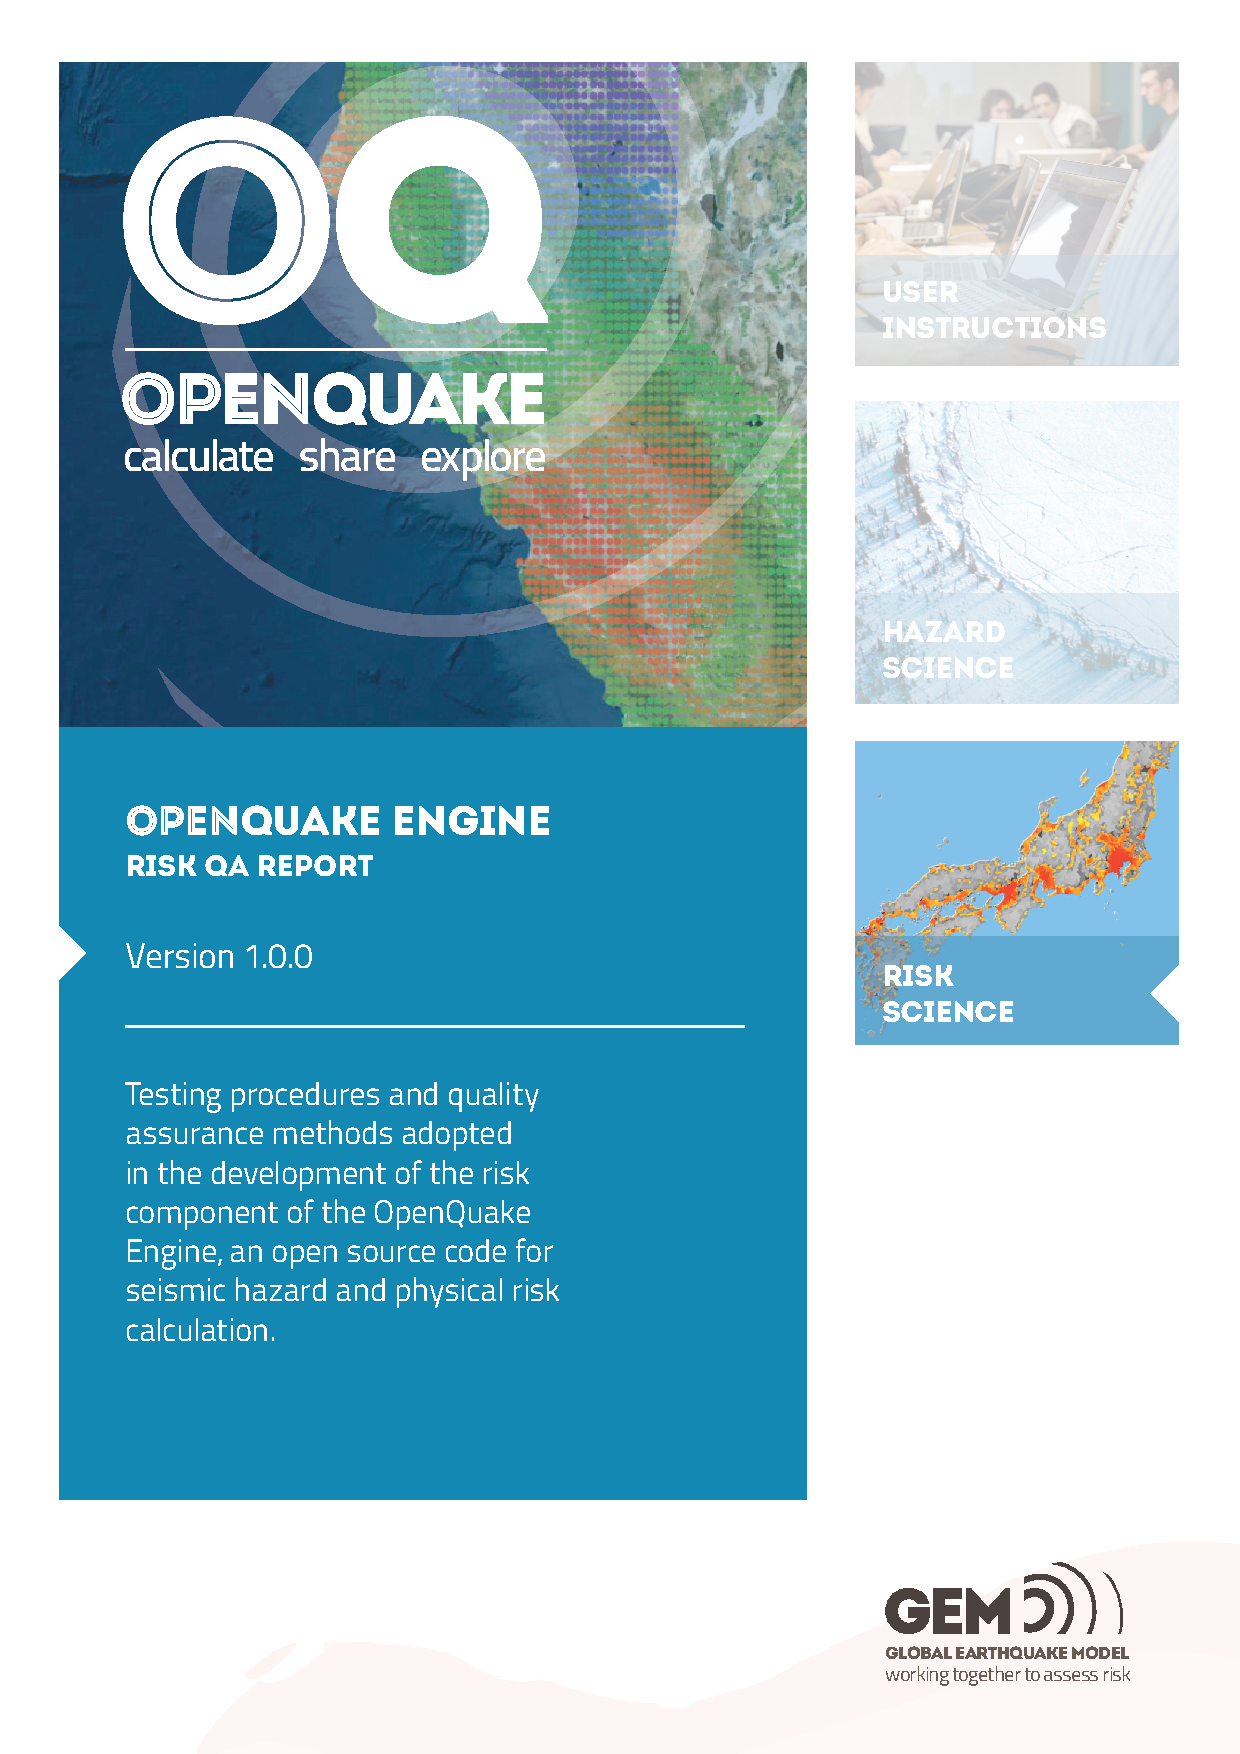
\includepdf[pages=-]{figures/oq-risk-qa-cover.pdf}

%-------------------------------------------------------------------------------
%  TITLE PAGE
%-------------------------------------------------------------------------------

\begingroup
\thispagestyle{empty}
%\AddToShipoutPicture*{\put(6,5){\includegraphics[scale=1]{background}}}
\par\normalfont\fontsize{15}{15}\sffamily\selectfont
“OpenQuake: Calculate, share, explore”
\centering
\vspace*{9cm}
\par\normalfont\fontsize{35}{35}\sffamily\selectfont
Testing procedures adopted in the development of the risk 
component of the OpenQuake-engine\par % Book title
\endgroup

%-------------------------------------------------------------------------------
%  COPYRIGHT PAGE
%-------------------------------------------------------------------------------

\newpage
~\vfill
\thispagestyle{empty}

\noindent
   \textbf{Authors} \\
   Anirudh Rao$^1$, Michele Simionato$^1$ \hfill \\
   \hfill \\
   \small
   \begin{tabular}{p{4cm}p{4cm}p{4cm}}
   $^1$ GEM Model Facility \hfill \newline
   via Ferrata, 1 \hfill \newline
   20133 Pavia \hfill \newline
   Italy \hfill \newline
   \end{tabular} \hfill \newline
   %
   Email address (for all the authors):\hfill\\
   $<$name.surname$>$@globalquakemodel.org\hfill\\
   \normalsize

\noindent \copyright\ \textsc{2015 GEM Foundation}\\ % Copyright notice
\noindent \textsc{globalquakemodel.org/openquake}\\ % URL
\noindent \hfill\\
\noindent
   {\textbf{Citation}} \hfill \\
   Please cite this document as: \hfill \\
   Rao, Anirudh and Simionato, Michele (2015). 
   Testing procedures adopted in the development of the risk 
   component of the OpenQuake-engine. 
   \textit{Global Earthquake Model (GEM) Technical Report 2015-07. 
   doi: 10.13117/GEM.OPENQUAKE.TR2015.07, 100 pages.} \hfill \\
\noindent \hfill\\
\noindent
   {\bf{Disclaimer}} \hfill \\
   This report is distributed in the hope that it will be 
   useful, but without any warranty: without even the implied warranty of 
   merchantability or fitness for a particular purpose. While every precaution 
   has been taken in the preparation of this document, in no event shall the 
   authors of the Manual and the GEM Foundation be liable to any party for 
   direct, indirect, special, incidental, or consequential damages, including 
   lost profits, arising out of the use of information contained in this 
   document or from the use of programs and source code that may accompany it, 
   even if the authors and GEM Foundation have been advised of the possibility 
   of such damage. The report provided hereunder is on as ``as is'' basis, and the 
   authors and GEM Foundation have no obligations to provide maintenance, 
   support, updates, enhancements, or modifications. \hfill \\
% \noindent
%    The current version of the report has been revised only by members of the 
%    GEM model facility and it must be considered a draft copy.
% \vspace{0.4cm} \hfill \\
\noindent \hfill\\
\noindent
   {\bf{License}} \hfill \\
   This report is distributed under the Creative Commons License 
   Attribution-NonCommercial-ShareAlike 4.0 International 
   (\href{http://creativecommons.org/licenses/by-nc-sa/4.0/}
   {CC BY-NC-SA 4.0}). 
   You can download this Manual and share it with 
   others as long as you provide proper credit, but you cannot change 
   it in any way or use it commercially.\hfill \\

\noindent \textit{First printing, July 2015} % Printing/edition date

%-------------------------------------------------------------------------------
%  TABLE OF CONTENTS
%-------------------------------------------------------------------------------

\chapterimage{figures/chapter_head_1.pdf} % Table of contents heading image
\pagestyle{empty} % No headers
\tableofcontents % Print the table of contents itself
\cleardoublepage % Forces the first chapter to start on the right
\pagestyle{fancy} % Print headers again

%-------------------------------------------------------------------------------
%  FOREWORD
%-------------------------------------------------------------------------------
% \chapterimage{figures/chapter_head_2.pdf} % Chapter heading image
% \chapter*{Preface}
% \addcontentsline{toc}{chapter}{Preface}
% \input{qareport/preamble.tex}

%-------------------------------------------------------------------------------
%  THE QA REPORT
%-------------------------------------------------------------------------------

% ------------------------------------------------------- Part I: Introduction -
\part{Introduction}

\chapterimage{figures/chapter_head_2.pdf} % Chapter heading image
\chapter{Software Testing}
   \label{chap:intro}
   The current document describes the extensive testing procedures adopted in the development of the risk component of the \gls{acr:oqe}, the open source hazard and risk software developed by the Global Earthquake Model initiative. A similar document describing the testing procedures for the hazard component of the engine is also available \citep{pagani2014_oqtesting}.

The OpenQuake risk library comprises a set of calculators capable of computing human or economic losses for a collection of assets, caused by a given scenario event, or by considering the probability of all possible events that might happen within a region within a certain time span.

The OpenQuake library comprises a set of calculators for assessing the potential economic losses and human casualties for a given ``scenario'' event or over a certain period of time. The outputs from the risk calculators may be used by disaster preparedness teams for gaining understanding about the potential consequences of an earthquake on a city, by structural engineers for evaluating the potential benefits of earthquake-resistant design or retrofitting and in the design of building codes, or by insurance and reinsurance firms for assessing the earthquake risk for a portfolio of assets.

These use cases clearly illustrate the need for rigorous testing and quality assurance of the software in question, and it is imperative that the implementation of the risk calculators be based on well-recognized, state-of-the-art and tested techniques; requirements that must be reconciled with the need to regularly incorporate recent advances given the progress carried out within the scientific community.

According to \citet{berkes2012} scientific software must be:
\begin{itemize}
\item Error proof
\item Flexible and able to accommodate different methods
\item Reproducible and re-usable
\end{itemize}

The features described below contribute to fulfill these requirements: %
\begin{itemize}
\item Software should have a modular and flexible structure capable of incorporating new features and - as a consequence - offer users the most recent and advanced techniques.
%
In very general terms, modularity is the level to which a component of a system can be moved, replaced or reused.
%
In software design, modularity means the separation of the software
into smaller independent components that can be implemented, maintained and tested easily and efficiently.
%
\item Software should have and extensive test coverage which captures possible errors and avoids regressions (i.e. unexpected behaviors introduced by new features).
%
Software testing \citep{myers2012} is an important, complex and vast discipline which helps in developing methods and processes aimed at certifying the extent to which a computer code behaves according to the original design intent and user specifications.
\end{itemize}

The \gls{acr:oqe} includes different levels of modularity. The first is the one separating the engine itself into a number of libraries, each one containing well identified knowledge, objects and methods (e.g. the OQ-hazardlib includes objects and methods needed to compute probabilistic seismic hazard and the OQ-risklib contains methods to compute scenario and probabilistic seismic risk). The second one pertains to the data model adopted in the development of each library as a result of the abstraction process.

\section{Testing and Quality Assurance}
\label{sec:intro-testing-qa}
Despite the distinction between software testing (in some cases also called Quality Control) and \gls{acr:sqa} being somewhat vague and partly open to personal judgment, it's clear that \gls{acr:sqa} is a more comprehensive and overarching process than software testing.
%
\gls{acr:sqa} aims at the definition of the best processes that should be used to provide guarantees that user expectations will be met.
%
Software testing focuses instead on detecting software faults by inspecting and testing the product at different stages of development.

% -----------------------------------------------------------------------------
\subsection{Software testing}
The basic purpose of software testing is to execute different parts of the program with the specific intent of finding errors or unexpected behavior.
%
The \gls{acr:oqe} and the associated libraries are developed following an agile paradigm. This development strategy is organized in a way that the creation of the real code is completed in parallel and fully integrated with the software testing process.

This type of testing of the OpenQuake risk (and hazard) library is achieved through extensive testing at various levels. At a very basic level, the introduction of any new code is always accompanied by a suite of unit-tests that check correct functioning of the new code for various combinations of possible inputs. Development also follows a continuous-integration approach, where the new code is merged into the codebase only after ensuring that the new code does not break any of the existing test cases.

All new code is also subject to a formal ``code-review'' process, where one or more programmers or scientists assess the new code both visually to check for logical errors, and through trial runs to verify that it functions as claimed.

% -----------------------------------------------------------------------------
\subsection{Quality assurance}
According to the IEEE ``Standard for Software Quality Assurance Processes'':
\emph{Software quality assurance is a set of activities that define and assess the adequacy of software processes to provide evidence that establishes confidence that the software processes are appropriate for and produce software products of suitable quality for their intended purposes. A key attribute of SQA is the objectivity of the SQA function with respect to the project. The SQA function may also be organizationally independent of the project; that is, free from technical, managerial, and financial pressures from the project.}

Thus, apart from the extensive set of unit-tests for individual functions and modules, the continuous-integration process and formal code-review practices, the OpenQuake risk calculators also have a set of quality assurance tests. The focus of these QA tests is to ensure that the calculators function according to specifications and that the results for specific input models produce the expected outputs. Chapter~4 of this report documents the full range of test cases employed in the QA testing of the OpenQuake risk calculators, along with descriptions of the expected results calculated by hand or using an alternate implementation of the calculators in the programming language Julia.



\section{Organization of the Report}
This document is organized into four chapters.

The current chapter provides a very brief and general introduction to software testing with a focus on the testing of scientific software.

The second chapter describes the module, or unit testing procedures adopted in the development of the \gls{acr:oqe} and we discuss some examples. The continuous integration mechanism used for development is also discussed.

The third chapter describes the general framework for the acceptance tests for the OpenQuake risk calculators. A brief overview of the theoretical background for the different calculators is also provided in this chapter.

The fourth chapter describes the different test cases, input models, and results for the acceptance tests implemented for the OpenQuake scenario risk, classical risk, and event-based risk calculators.

% In the fifth chapter, we compare the loss curves computed using the event-based calculator with the corresponding loss curves computed using the classical-PSHA based calculator.

% In the sixth chapter, we illustrate tests comparing the results computed with the \gls{acr:oqe} against the ones computed using different probabilistic seismic risk analysis software.

% Chapter seven describes the OpenQuake risk demos and the average 

% The final chapter describes the set of 

% -------------------------------------------------------- Part II: Unit Tests -
\thispagestyle{empty}
\part{Unit Tests}

\chapterimage{figures/chapter_head_2.pdf} % Chapter heading image
\chapter{Unit Testing in the OpenQuake-engine}
   \label{chap:unit-tests}
   This chapter provides an introduction to the module (unit) testing procedures \citep{myers2012} and describes the estensive series of tests implemented in the \gls{acr:oqe}.

\section{Overview of Unit-Testing}
\label{sec:ut-overview}
At the first level of the code testing process is the practice of
``unit-testing''. This process is a central tenet of test-driven software
development and is widely established as a means of ``best-practice''. %
Before looking closely at the OpenQuake-engine
approach to unit-testing it is important to establish what are the precise objectives of the unit-testing process and the benefits (and limitations) that it brings.


\subsection{Correctness of implementation}
This objective is obviously the primary goal of unit-testing, to ensure that each function of the code is operating in the manner expected by the developer. ``Correctness'', in this case, requires that the function produces both the correct output, but also if there are cases in which function may fail then the means of failure should be predictable. The following is a relatively simple example of how a unit-test relates to a function:

Consider a simple function to multiply two numbers and take the logarithm of the result. A relevant analogy may be that of a magnitude scaling relation calculation, in which both a rupture length and rupture width are required, and the logarithm of the area may be needed by the function itself. In this circumstance a negative value in either of the two inputs would result in a calculation error. This could be coded in the following manner:

\begin{lstlisting}[frame=single]
def get_log_area(length, width):
    if (length < 0) or (width < 0):
        raise valueError("Both inputs must be positive")
    else:
        return log10(length * width)
\end{lstlisting}

From the description above it is evident that the user requirements  inform the manner in which the function should behave (i.e. negative
values cannot be tolerated). To ensure that the function is operating
correctly, we wish to write a set of tests that will confirm the behaviour is correct:

\begin{enumerate}
\item If both $a$ and $b$ are equal to 10.0, then the function     should return 2.0
\item If $a = -1$ and $b = 10$ the function should raise an error     reporting the stated message ``Both inputs must be positive''.
\item If $a = 10$ and $b = -1$ the function should raise an error     reporting the stated message ``Both inputs must be positive''.
\item If $a = -1$ and $b = -1$ the function should raise an error     reporting the stated message ``Both inputs must be positive''.
\end{enumerate}

A unit-test for this function is an additional function that will check that both cases are satisfied, and will report an error if not. 
A comprehensive unit-test suite for a software may fulfil two objectives: \textbf{line coverage} and \textbf{parameter coverage}. The former should ensure that, in as far as possible, every line (or statement) in the code is executed at some point in the testing process. The latter should ensure
that the behaviour of the function is predictable when supplied with ``unusual'' parameters. In the above example, both objectives are satisfied
by the tests. The first test will result in a positive valued ``area'',
thus executing the second branch of the logical path, the second test will
result in a negative area and will execute the first logical branch. %
Therefore all lines of the code are covered and the line coverage is complete. We also see that in this simple example there are four possible
cases: i) a is positive and b is positive, ii) a is positive and b is negative,  ii) a is negative and b is positive, and iv) both a and b are negative. Only the first case is valid, therefore the first test ensures that they provide the correct answer (usually verified by independent means), whilst the remaining tests should ensure that the function raises the correct error. Thus the full parameter space of the input is ensured.

The above case is, of course, trivial; however, as shall be seen in due
course, this same process can be applied in more complex contexts.

Furthermore, the same unit-testing approach can be applied not only to individual components within the PSHA calculation, but also to full calculations, essentially verifying that the hazard curve produced by the full PSHA calculator is in agreement with that produced independently (sometimes by hand).


\subsection{Identify problems prior to software release}
This advantage is largely self-explanatory, but for many software projects this can reduce the possibility of requiring \emph{a posteriori} fixes to
the code (patches). By compiling a comprehensive suite of unit-tests, and following a software development and release process that should automatically run the tests at the point of packaging, this should ensure that new features added to the software cannot inadvertently break other components.


\subsection{Facilitate improvements in performance}
In the creation of software intended to perform demanding scientific calculations, like those commonly associated with PSHA, the issue of computational performance and efficiency is a major one. There is a continuing need to improve the speed and reduce the work required to undertake the PSHA calculation. To implement improvements it is necessary to ensure that optimisations do not modify the outputs of the calculation, only the speed at which they are performed. The unit-testing is absolutely fundamental to this process as optimisation cannot be undertaken readily without a means to ensure the calculation outputs have not changed. This point was a critical motivation behind the transition from the OpenSHA basis of the OpenQuake hazard calculation engine prior to version 1.0, to the current OpenQuake hazard library.


\section{Continuous Integration}
\label{sec:ut-ci}
\gls{acr:oqe} is developed and packaged within a ``continuous integration'' system (\href{https://ci.openquake.org/}{https://ci.openquake.org/}),
based on the open-source software ``Jenkins'' (\href{http://jenkins-ci.org/}{http://jenkins-ci.org/}). Continuous integration is used in large software projects to run a full test suite of the complete software, either at fixed time intervals or, as in the current case, when any new code is committed to the repository. The continuous integration system does the following:

\begin{enumerate}
\item Run the full set of unit-tests for all code in all of the linked repositories. This will include the main (or ``master'') branch of the software repository, i.e. the one that will be used for packaging of the software, as well as some development branches.
\item Run a test of the software installation. This test will install the software on a dedicated platform and check that the installation of the software is successful. This test also ensures that if changes occur in the dependency packages, and these changes affect or compromise the installation and operation of the software, these problems are recognised immediately.
\item The software will also run standard Python tests for quality of code, compilation of documentation etc.
\item Several long-running tests may also be run. These implement larger scale seismic hazard and risk calculations designed to test the overall performance of the engine.
\end{enumerate}

If at any point the tests should fail, the OpenQuake development team will be notified automatically. This ensures that software that is failing any of the tests will remain on the main branch of the repository for the minimum amount of time possible. Furthermore, if the continuous integration tests fail, the new code will not be integrated into the nightly package of the software.

\section{Unit-Tests in the OpenQuake Risk Library}
\label{sec:ut-risklib}
\subsection{Component level tests}
The unit-testing at the component level breaks the functions into simple
calculations whose results can be verified by hand. These tests, similar in nature to that illustrated previously, provide the majority of the line and parameter coverage needed to ensure a robust code.

To illustrate the comprehensive nature of the coverage we consider the example of 
%
The test suite for this one function is illustrative of several key components of the unit-testing. First is the use of an independent tool to provide the expected values of the calculation under simple conditions. Second is the use of ``extreme cases'' such as polar locations, or across the International Dateline. These ensure that the function can be global in application.

The nature of the interdependencies between the functions also means that one a functions own unit-test is verified, the function can then form the basis for testing other conditions. So for example, the geodetic distance tools also contain a method to calculate the minimum distance between a collection of points and a single point. Rather than requiring new expected distances for the different conditions, the geodetic distance function can then be used to construct tests for functions that utilise it. This makes the testing process more efficient, and reduces the need to write large numbers of tests in order to ensure correct behaviour of the function.

\section{Summary}
\label{sec:ut-summary}
In this chapter we have outlined both the process and the key benefits of developing comprehensive unit-tests for OpenQuake-engine, as well as outlining the operation of the continuous integration system, which should ensure that code with the potential to break the tests cannot be packaged and released. The unit-tests themselves have not been discussed in detail as nearly one thousand tests are executed during the unit-test process. However, to view the comprehensive set of tests, the reader is encouraged to refer to the full test-suite, which is open and available on the OpenQuake code repository (\href{https://github.com/gem/oq-risklib/tree/master/openquake/risklib/tests}
{https://github.com/gem/oq-risklib/tree/master/openquake/risklib/tests}).

Furthermore, we have also discussed how the OpenQuake-engine development tries to facilitate correct implementation of features such as ground motion prediction equations. For relatively simple conditions, a selection of PEER tests \citep{thomas2010} are built into the testing process, making OpenQuake-engine unique amongst other hazard software in integrating the verification into the development process.

The following chapters will expand in greater detail upon the additional loss curve benchmark tests, which both follow and expand upon the PEER testing process.

   \cleardoublepage

% ------------------------------------------------- Part III: Acceptance Tests -
\thispagestyle{empty}
\part{Acceptance Tests}

\chapterimage{figures/chapter_head_2.pdf} % Chapter heading image
\chapter{Framework for Acceptance Testing}
   \label{chap:acc-framework}
   \section{Verification Framework}
The main purpose of the acceptance tests is to ensure that the risk calculators work according to the design specifications and to verify that the calculators produce correct results for a variety of input cases. Correctness of the test case results is verified by comparing with hand calculations for the simple test cases or with alternate implementaions in Julia for the complex cases.

\section{Theoretical Background}
\subsection{Basic concepts}
   \label{subsec:theory-basic-concepts}
   % Rupture
% GMF
% SES
% VF
% FF
% HC
% Monte Carlo
% GMPE

An earthquake \textit{rupture model} describes the magnitude, geometry, and source typology of an earthquake occurrence.

Given an earthquake rupture, the simulation of ground shaking values on a set of locations $\bm{x}=(x_{1}, x_{2}, ..., x_{N})$
forms a \textit{ground motion field} ($GMF$). The ground motion field is simulated by sampling the probability distribution defined by the ground motion model.

Seismicity in a region is described by a seismic source model ($SSM$), which is a collection of \textit{independent seismic sources}. Independence of seismic sources implies that the occurrence of an earthquake rupture in a source does not affect the probability of earthquake occurrence in the other sources.

The main parameters describing a seismic source are the geometry constraining the earthquake rupture locations, and the \textit{magnitude-frequency distribution}, defining the average annual occurrence rate over a magnitude range. A seismic source model ($SSM$) can be therefore defined as a set of $I$ seismic sources ($Src$):
\begin{equation}
SSM = \left\{Src_{1}, Src_{2}, ..., Src_{I}\right\}
\end{equation}

Each source generates \textit{independent earthquake ruptures}. Independence of earthquake ruptures implies that the occurrence of an earthquake rupture in a source does not affect the probability of occurrence of the other potential earthquake ruptures in the same source. A generic $i$-th source defines therefore a set of $J$ earthquake ruptures:
\begin{equation}
Src_{i} = \left\{Rup_{i1}, Rup_{i2}, ..., Rup_{iJ}\right\}
\end{equation}





Probabilistic seismic hazard analysis allows calculating the probabilities of exceeding,
at least once in a given time span, and at a given site, a set of ground motion
parameter levels considering all possible earthquake ruptures defined in a
seismic source model. Such a list of probability values is usually referred to
as \textit{hazard curve}.


\subsection{Scenario risk}
   \label{subsec:theory-scenario-risk}
   The scenario risk calculator computes loss statistics for all assets in a given exposure model for a single specified earthquake rupture. Loss statistics include the mean and standard deviation of ground-up losses and insured losses for each loss type considered in the analysis. Loss statistics can currently be computed for five different loss types using this calculator: structural losses, nonstructural losses, contents losses, downtime losses, and occupant fatalities. This calculator requires the definition of a finite rupture model, an exposure model and a vulnerability model for each loss type considered; the main results are the loss statistics per asset and mean loss maps.

The rupture characteristics—i.e. the magnitude, hypocenter and fault geometry—are modelled as deterministic in the scenario calculators. Multiple realizations of different possible ground motion fields (GMFs) due to the single rupture are generated, taking into consideration both the inter-event variability of ground motions, and the intra-event residuals obtained from a spatial correlation model for ground motion residuals. The use of logic-trees allows for the consideration of uncertainty in the choice of a GMPE model for the given tectonic region and in the choice of vulnerability functions for the different taxonomy types in the exposure model.

As an alternative to computing the GMFs with OpenQuake, users can also provide their own sets of GMFs as input to the scenario risk calculator.

For each GMF realization, a loss ratio is sampled for every asset in the exposure model using the provided probabilistic vulnerability model, taking into consideration the correlation model for vulnerability of different assets of a given taxonomy. Finally loss statistics, i.e., the mean loss and standard deviation of loss for both ground-up losses and insured losses across all realizations, are calculated for each asset. Mean loss maps are also generated by this calculator, describing the mean ground-up losses and mean insured losses caused by the scenario event for the different assets in the exposure model.

\subsection{Scenario damage}
   \label{subsec:theory-scenario-damage}
   The scenario damage calculator computes damage distribution statistics for all assets in a given exposure model for a single specified earthquake rupture. Damage distribution statistics include the mean and standard deviation of damage fractions for different damage states. This calculator requires the definition of a finite rupture model, an exposure model and a fragility model; the main results are the damage distribution statistics per asset, aggregated damage distribution statistics per taxonomy, aggregated damage distribution statistics for the region, and collapse maps.

The rupture characteristics—i.e. the magnitude, hypocenter and fault geometry—are modelled as deterministic in the scenario calculators. Multiple realizations of different possible ground motion fields (GMFs) due to the single rupture are generated, taking into consideration both the inter-event variability of ground motions, and the intra-event residuals obtained from a spatial correlation model for ground motion residuals. The use of logic-trees allows for the consideration of uncertainty in the choice of a GMPE model for the given tectonic region and in the choice of fragility functions for the different taxonomy types in the exposure model.

As an alternative to computing the GMFs with OpenQuake, users can also provide their own sets of GMFs as input to the scenario damage calculator.

For each GMF realization, damage fractions (the fraction of buildings in each damage state) are estimated for every asset in the exposure model using the provided fragility model, and finally the damage distribution statistics (i.e., the mean damage fractions and standard deviation of damage fractions for all damage states) across all realizations are calculated. The calculator also provides aggregated damage distribution statistics for the portfolio, such as mean damage fractions and standard deviation of damage fractions for each taxonomy in the exposure model, and the mean damage fractions and standard deviation of damage fractions for the entire region of study.
\subsection{Classical PSHA-based risk}
   \label{subsec:theory-classical-risk}
   The classical PSHA-based risk calculator convolves through numerical integration, the probabilistic vulnerability functions for an asset with the seismic hazard curve at the location of the asset, to give the loss distribution for the asset within a specified time period. The calculator requires the definition of an exposure model, a vulnerability model for each loss type of interest with vulnerability functions for each taxonomy represented in the exposure model, and hazard curves calculated in the region of interest. Loss curves and loss maps can currently be calculated for five different loss types using this calculator: structural losses, nonstructural losses, contents losses, downtime losses, and occupant fatalities. The main results of this calculator are loss exceedance curves for each asset, which describe the probability of exceedance of different loss levels over the specified time period, and loss maps for the region, which describe the loss values that have a given probability of exceedance over the specified time period.

The hazard curves required for this calculator can be calculated by the OpenQuake engine for all asset locations in the exposure model using the classical PSHA approach (Cornell, 1968; McGuire, 1976). The use of logic-trees allows for the consideration of uncertainty in the choice of a GMPE model for the different tectonic region types in the region and in the choice of vulnerability functions for the different taxonomy types in the exposure model.

\subsection{Classical PSHA-based damage}
   \label{subsec:theory-classical-damage}
   The classical PSHA-based risk calculator convolves through numerical integration, the probabilistic vulnerability functions for an asset with the seismic hazard curve at the location of the asset, to give the loss distribution for the asset within a specified time period. The calculator requires the definition of an exposure model, a vulnerability model for each loss type of interest with vulnerability functions for each taxonomy represented in the exposure model, and hazard curves calculated in the region of interest. Loss curves and loss maps can currently be calculated for five different loss types using this calculator: structural losses, nonstructural losses, contents losses, downtime losses, and occupant fatalities. The main results of this calculator are loss exceedance curves for each asset, which describe the probability of exceedance of different loss levels over the specified time period, and loss maps for the region, which describe the loss values that have a given probability of exceedance over the specified time period.

The hazard curves required for this calculator can be calculated by the OpenQuake engine for all asset locations in the exposure model using the classical PSHA approach (Cornell, 1968; McGuire, 1976). The use of logic-trees allows for the consideration of uncertainty in the choice of a GMPE model for the different tectonic region types in the region and in the choice of vulnerability functions for the different taxonomy types in the exposure model.

\subsection{Event-based risk}
   \label{subsec:theory-eventbased}
   This calculator employs an event-based Monte Carlo simulation approach to probabilistic risk assessment in order to estimate the loss distribution for individual assets and aggregated loss distribution for a spatially distributed portfolio of assets within a specified time period. The calculator requires the definition of an exposure model, a vulnerability model for each loss type of interest with vulnerability functions for each taxonomy represented in the exposure model, and a set of ground motion fields representative of the seismicity of the region over the specified time period. Loss curves and loss maps can currently be calculated for five different loss types using this calculator: structural losses, nonstructural losses, contents losses, downtime losses, and occupant fatalities. The main results of this calculator are loss exceedance curves for each asset, which describe the probability of exceedance of different loss levels over the specified time period, and loss maps for the region, which describe the loss values that have a given probability of exceedance over the specified time period. Aggregate loss exceedance curves can be also be produced using this calculator; these describe the probability of exceedance of different loss levels for all assets of a single taxonomy, or for all assets in the portfolio, over the specified time period. Finally, event loss tables can be produced using this calculator; these tables describe the total loss across the portfolio for each seismic event in the stochastic event set.

This calculator relies on the probabilistic event-based hazard calculator, which simulates the seismicity of the chosen time period $T$ by producing a \textit{stochastic event set} (also known as a \textit{synthetic catalog}). For each rupture generated by a source, the number of occurrences in the given time span $T$ is simulated by sampling the corresponding probability distribution as given by $P_{rup}(k | T)$. A stochastic event set is therefore a \textit{sample} of the full population of ruptures as defined by a seismic source model. Each rupture is present zero, one or more times, depending on its probability. Symbolically, we can define a stochastic event set ($SES$) as:
\begin{align}
SES(T) = \left\{k \times rup,\;k\sim P_{rup}(k | T)\;\;\forall\;rup\;in\;Src\;\forall\;Src\;in\;SSM\right\}
\end{align}
where $k$, the number of occurrences, is a random sample of $P_{rup}(k | T)$, and $k \times rup$ means that rupture $rup$ is repeated $k$ times in the stochastic event set.

For each event in the stochastic event sets, a spatially correlated ground motion field (GMF) realisation is generated, taking into consideration both the inter-event variability of ground motions, and the intra-event residuals obtained from a spatial correlation model for ground motion residuals. The use of logic-trees allows for the consideration of uncertainty in the choice of a seismic source model, in the choice of GMPE models for the different tectonic regions, and in the choice of vulnerability functions for the different taxonomy types in the exposure model.

For each GMF realization, a loss ratio is sampled for every asset in the exposure model using the provided probabilistic vulnerability model, taking into consideration the correlation model for vulnerability of different assets of a given taxonomy. Finally loss exceedance curves are computed for both ground-up losses and insured losses.
   \cleardoublepage
   \cleardoublepage
\chapter{Test Cases and Results}
   \label{chap:acc-tests}
   \section{Scenario Risk Calculator}
   \label{sec:acc-sr}
   The tests for the scenario risk calculator assume the correct computation of the ground motion fields at the locations of the assets in the exposure model. Thus, the risk tests implicitly rely on the acceptance tests for the scenario hazard calculator.

The rupture model used for the tests comprises a magnitude $M_W 6.7$ rupture on a vertical strike-slip fault.\\

\noindent Details of the rupture are given below:\\

\noindent
Fault type: Strike slip\\
Fault dip: $90^{\circ}$\\
Fault plane depths: 0--20 km\\
Fault coordinates:\\
South end: $38.0000^{\circ} N$, $122.0000^{\circ} W$\\
North end: $38.2248^{\circ} N$, $122.0000^{\circ} W$\\
Rupture magnitude: 6.7\\
Rupture hypocenter: $38.1124^{\circ} N$, $122.0000^{\circ} W$\\
Hypocenter depth: 10 km\\

The complete collection of input models and job configuration files used in these test cases can be accessed here:
\href{https://github.com/gem/oq-risklib/tree/master/openquake/qa_tests_data/scenario_risk}
{https://github.com/gem/oq-risklib/tree/master/openquake/qa\_tests\_data/scenario\_risk}

\subsection{Single asset tests}
\label{subsec:acc-sr-single}
The single asset test cases are designed to test the basic elements of the scenario risk calculator, such as:

\begin{itemize}
\item basic loss field computation
\item calculation of mean and standard deviation of scenario loss
\end{itemize}

\input{qareport/tables/tab-asset.tex}

The location and taxonomy of the single asset in the exposure model used for the single-asset test cases for the scenario risk calculator are given in Table \ref{tab:asset}.

% ---------------------------------------------------------------------------
\subsubsection{Case 1a}
\input{qareport/cases/sr-1a}
\input{qareport/results/sr-1a}
Table \ref{tab:result-sr-1a} shows the comparison of the OpenQuake result with the expected result.

% ---------------------------------------------------------------------------
\subsubsection{Case 1b}
\input{qareport/cases/sr-1b}
\input{qareport/results/sr-1b}
Table \ref{tab:result-sr-1b} shows the comparison of the OpenQuake result with the expected result.

% ---------------------------------------------------------------------------
\subsubsection{Case 1c}
\input{qareport/cases/sr-1c}
\input{qareport/results/sr-1c}
Table \ref{tab:result-sr-1c} shows the comparison of the OpenQuake result with the expected result.

% ---------------------------------------------------------------------------
\subsubsection{Case 1d}
\input{qareport/cases/sr-1d}
\input{qareport/results/sr-1d}
Table \ref{tab:result-sr-1d} shows the comparison of the OpenQuake result with the expected result.

% ---------------------------------------------------------------------------
\subsubsection{Case 1e}
\input{qareport/cases/sr-1e}
\input{qareport/results/sr-1e}
Table \ref{tab:result-sr-1e} shows the comparison of the OpenQuake result with the expected result.

% ---------------------------------------------------------------------------
\subsubsection{Case 1f}
\input{qareport/cases/sr-1f}
\input{qareport/results/sr-1f}
Table \ref{tab:result-sr-1f} shows the comparison of the OpenQuake result with the expected result.

% ---------------------------------------------------------------------------
\subsubsection{Case 1g}
\input{qareport/cases/sr-1g}
\input{qareport/results/sr-1g}
Table \ref{tab:result-sr-1g} shows the comparison of the OpenQuake result with the expected result.

% ---------------------------------------------------------------------------
\subsubsection{Case 1h}
\input{qareport/cases/sr-1h}
\input{qareport/results/sr-1h}
Table \ref{tab:result-sr-1h} shows the comparison of the OpenQuake result with the expected result.

% ---------------------------------------------------------------------------
\subsubsection{Case 2a}
\input{qareport/cases/sr-2a}
\input{qareport/results/sr-2a}
Table \ref{tab:result-sr-2a} shows the comparison of the OpenQuake result with the expected result.

% ---------------------------------------------------------------------------
\subsubsection{Case 2b}
\input{qareport/cases/sr-2b}
\input{qareport/results/sr-2b}
Table \ref{tab:result-sr-2b} shows the comparison of the OpenQuake result with the expected result.

% ---------------------------------------------------------------------------
\subsubsection{Case 2c}
\input{qareport/cases/sr-2c}
\input{qareport/results/sr-2c}
Table \ref{tab:result-sr-2c} shows the comparison of the OpenQuake result with the expected result.

% ---------------------------------------------------------------------------
\subsubsection{Case 2d}
\input{qareport/cases/sr-2d}
\input{qareport/results/sr-2d}
Table \ref{tab:result-sr-2d} shows the comparison of the OpenQuake result with the expected result.

% ---------------------------------------------------------------------------
\subsubsection{Case 3a}
\input{qareport/cases/sr-3a}
\input{qareport/results/sr-3a}
Table \ref{tab:result-sr-3a} shows the comparison of the OpenQuake result with the expected result.

% ---------------------------------------------------------------------------
\subsubsection{Case 3b}
\input{qareport/cases/sr-3b}
\input{qareport/results/sr-3b}
Table \ref{tab:result-sr-3b} shows the comparison of the OpenQuake result with the expected result.
% ---------------------------------------------------------------------------
\subsubsection{Case 3c}
\input{qareport/cases/sr-3c}
\input{qareport/results/sr-3c}
Table \ref{tab:result-sr-3c} shows the comparison of the OpenQuake result with the expected result.

% ---------------------------------------------------------------------------
\subsubsection{Case 3d}
\input{qareport/cases/sr-3d}
\input{qareport/results/sr-3d}
Table \ref{tab:result-sr-3d} shows the comparison of the OpenQuake result with the expected result.


% -----------------------------------------------------------------------------
\subsection{Multiple asset tests}
\label{subsec:acc-sr-multiple}
The multiple asset test cases are designed to test the loss aggregation functions of the scenario risk calculator, such as:

\begin{itemize}
\item portfolio loss computation for a given ground motion field
\item calculation of mean and standard deviation of portfolio scenario loss
\end{itemize}

\input{qareport/tables/tab-assets.tex}

The list of assets in the exposure model used for the multiple-asset test cases for the scenario risk calculator is given in Table \ref{tab:assets}.

Ten thousand ground motion fields are generated for the given rupture, taking into consideration both the inter-event and intra-event variability in the ground motion. The ground motion prediction equation used is Boore and Atkinson (2008), and the Jayaram and Baker (2009) model for spatial correlation of ground motion values is applied.

\input{qareport/tables/tab-scenario-gmfs-multiple}

Table \ref{tab:scenario-gmfs-multiple} lists three of the ten thousand ground motion fields generated.

% ---------------------------------------------------------------------------
\subsubsection{Case 5a}
The purpose of this case is to test the computation of the mean and standard deviation of the loss for multiple assets, given variability in both the ground motion values and in the vulnerability function. The computation of the mean and standard deviation of the portfolio loss is also tested in this case. The asset vulnerability correlation factor is zero for this test case.


\input{qareport/results/tab-result-scenario-risk-5a}

Table \ref{tab:result-scenario-risk-5a} shows the comparison of the OpenQuake result with the expected result.

% ---------------------------------------------------------------------------
\subsubsection{Case 5b}


\input{qareport/results/tab-result-scenario-risk-5b}

Table \ref{tab:result-scenario-risk-5b} shows the comparison of the OpenQuake result with the expected result.

% ---------------------------------------------------------------------------
\subsubsection{Case 5c}


\input{qareport/results/tab-result-scenario-risk-5c}

Table \ref{tab:result-scenario-risk-5c} shows the comparison of the OpenQuake result with the expected result.

% ---------------------------------------------------------------------------
\subsubsection{Case 5d}


\input{qareport/results/tab-result-scenario-risk-5d}

Table \ref{tab:result-scenario-risk-5d} shows the comparison of the OpenQuake result with the expected result.

% ---------------------------------------------------------------------------

% -----------------------------------------------------------------------------
\subsection{Calculation with logic-trees}
\label{subsec:acc-sr-lt}
\subsubsection{Case 6a}


\input{qareport/results/tab-result-scenario-risk-6a}

Table \ref{tab:result-scenario-risk-6a} shows the comparison of the OpenQuake result with the expected result.

% ---------------------------------------------------------------------------


% -----------------------------------------------------------------------------
\subsection{Insurance tests}
\label{subsec:acc-sr-insurance}
\subsubsection{Case 5a}
\input{qareport/cases/sr-5a}
\input{qareport/results/sr-5a}
Table \ref{tab:result-sr-5a} shows the comparison of the OpenQuake result with the expected result.
\section{Scenario Damage Calculator}
   \label{sec:acc-sd}
   The tests for the scenario damage calculator assume the correct computation of the ground motion fields at the locations of the assets in the exposure model. Thus, the risk quality assurance tests implicitly rely on the acceptance tests for the scenario hazard calculator.

The rupture model used for the tests comprises a magnitude $M6.7$ rupture on a vertical strike-slip fault, the same as is used in the tests for the scenario risk calculator.\\

\noindent Details of the rupture are repeated below for convenience:\\

\noindent
Fault type: Strike slip\\
Fault dip: $90^{\circ}$\\
Fault plane depths: 0--20 km\\
Fault coordinates:\\
South end: $38.0000^{\circ} N$, $122.0000^{\circ} W$\\
North end: $38.2248^{\circ} N$, $122.0000^{\circ} W$\\
Rupture magnitude: 6.7\\
Rupture hypocenter: $38.1124^{\circ} N$, $122.0000^{\circ} W$\\
Hypocenter depth: 10 km\\

The complete collection of input models and job configuration files used in these test cases can be accessed here:
\href{https://github.com/gem/oq-risklib/tree/master/openquake/qa_tests_data/scenario_damage}
{https://github.com/gem/oq-risklib/tree/master/openquake/qa\_tests\_data/scenario\_damage}

\subsection{Single asset tests}
\label{subsec:acc-sd-single}
The single asset test cases are designed to test the basic elements of the scenario damage calculator, such as:

\begin{itemize}
\item interpolation of the discrete fragility functions
\item damage distribution computation for a given set of ground motion fields
\item extraction of the probability of collapse
\end{itemize}

The location and taxonomy of the single asset in the exposure model used for the single-asset test cases for the scenario risk calculator are given in Table~\ref{tab:asset}.

% ---------------------------------------------------------------------------
\subsubsection{Case 1a}
\input{qareport/cases/sd-1a}
\input{qareport/results/sd-1a}
Table \ref{tab:result-sd-1a} shows the comparison of the OpenQuake result with the expected result.

% ---------------------------------------------------------------------------
\subsubsection{Case 1b}
\input{qareport/cases/sd-1b}
\input{qareport/results/sd-1b}
Table \ref{tab:result-sd-1b} shows the comparison of the OpenQuake result with the expected result.

% ---------------------------------------------------------------------------
\subsubsection{Case 1c}
\input{qareport/cases/sd-1c}
\input{qareport/results/sd-1c}
Table \ref{tab:result-sd-1c} shows the comparison of the OpenQuake result with the expected result.

% ---------------------------------------------------------------------------
\subsubsection{Case 1d}
\input{qareport/cases/sd-1d}
\input{qareport/results/sd-1d}
Table \ref{tab:result-sd-1d} shows the comparison of the OpenQuake result with the expected result.
% ---------------------------------------------------------------------------
\subsubsection{Case 1e}
\input{qareport/cases/sd-1e}
\input{qareport/results/sd-1e}
Table \ref{tab:result-sd-1e} shows the comparison of the OpenQuake result with the expected result.
% ---------------------------------------------------------------------------
\subsubsection{Case 1f}
\input{qareport/cases/sd-1f}
\input{qareport/results/sd-1f}
Table \ref{tab:result-sd-1f} shows the comparison of the OpenQuake result with the expected result.
% ---------------------------------------------------------------------------
\subsubsection{Case 1g}
\input{qareport/cases/sd-1g}
\input{qareport/results/sd-1g}
Table \ref{tab:result-sd-1g} shows the comparison of the OpenQuake result with the expected result.

% -----------------------------------------------------------------------------
% \subsection{Multiple asset tests}
% \label{subsec:acc-sd-multiple}
% The multiple asset test cases are designed to test the loss aggregation functions of the scenario damage calculator, such as:

\begin{itemize}
\item damage distribution per taxonomy
\item damage distribution for the portfolio
\end{itemize}

The list of assets in the exposure model used for the multiple-asset test cases for the scenario damage calculator is given in Table \ref{tab:assets}.






% -----------------------------------------------------------------------------
\subsection{Calculation with logic-trees}
\label{subsec:acc-sd-lt}
% ---------------------------------------------------------------------------
\subsubsection{Case 3a}
\input{qareport/cases/sd-3a}
\input{qareport/results/sd-3a}

Table \ref{tab:result-sd-3a} shows the comparison of the OpenQuake results with the expected results.

\section{Classical Risk Calculator}
   \label{sec:acc-cr}
   The tests for the classical PSHA-based risk calculator assume the correct computation of the hazard curves at the locations of the assets in the exposure model. Thus, the risk tests implicitly rely on the acceptance tests for the classical PSHA-based hazard calculator.

The source model used for the tests comprises a single vertical strike-slip fault with a Gutenberg-Richter b-value equal to 0.9 and a slip rate of 2 mm/yr. The MFD is a Gutenberg-Richter distribution truncated between magnitudes 5.0 and 6.5, while the Ground Motion Prediction Equation (GMPE) used is \citet{boore2008}.\\

\noindent Details of the fault geometry are given below:\\

\noindent
Fault type: Strike slip\\
Fault dip: $90^{\circ}$\\
Fault plane depths: 0--12 km\\
Fault coordinates:\\
South end: $38.0000^{\circ} N$, $122.0000^{\circ} W$\\
North end: $38.2248^{\circ} N$, $122.0000^{\circ} W$\\

Figure~\ref{fig:fault-sites}, shows the fault described above and the site geometry for the test cases described in the following sections. The single asset tests use only site $1$ shown in the figure, whereas the multiple asset tests use all seven of the sites.

\begin{figure}[htbp]
\centering
\includegraphics[width=12cm]{qareport/figures/fig-fault-site}
\caption{Fault and site geometry for the classical risk tests}
\label{fig:fault-site}
\end{figure}

The complete collection of input models and job configuration files used in these test cases can be accessed here:
\href{https://github.com/gem/oq-risklib/tree/master/openquake/qa_tests_data/classical_risk}
{https://github.com/gem/oq-risklib/tree/master/openquake/qa\_tests\_data/classical\_risk}

\subsection{Single asset tests}
\label{subsec:acc-cr-single}
The single asset test cases are designed to test the basic elements of the classical-PSHA based risk calculator, such as:

\begin{itemize}
\item asset loss ratio exceedance curve computation
\item asset loss exceedance curve computation
\end{itemize}

The location and taxonomy of the single asset in the exposure model used for the single-asset test cases for the classical risk calculator are given in Table \ref{tab:assets}.

% ---------------------------------------------------------------------------
\subsubsection{Case 1a}
\input{qareport/cases/cr-1a}
\input{qareport/results/tab-result-cr-1a}
Table \ref{tab:result-cr-1a} shows the comparison of the OpenQuake result with the expected result.

% ---------------------------------------------------------------------------
\subsubsection{Case 1b}
Test case 1b 

\input{qareport/results/tab-result-classical-risk-1b}

Table \ref{tab:result-classical-risk-1b} shows the comparison of the OpenQuake result with the expected result.

% ---------------------------------------------------------------------------
\subsubsection{Case 1c}


\input{qareport/results/tab-result-classical-risk-1c}

Table \ref{tab:result-classical-risk-1c} shows the comparison of the OpenQuake result with the expected result.

% ---------------------------------------------------------------------------
\subsubsection{Case 1d}


\input{qareport/results/tab-result-classical-risk-1d}

Table \ref{tab:result-classical-risk-1d} shows the comparison of the OpenQuake result with the expected result.

% ---------------------------------------------------------------------------
\subsubsection{Case 1e}


\input{qareport/results/tab-result-classical-risk-1e}

Table \ref{tab:result-classical-risk-1e} shows the comparison of the OpenQuake result with the expected result.

% ---------------------------------------------------------------------------
\subsubsection{Case 2a}


\input{qareport/results/tab-result-classical-risk-2a}

Table \ref{tab:result-classical-risk-2a} shows the comparison of the OpenQuake result with the expected result.

% ---------------------------------------------------------------------------
\subsubsection{Case 2b}


\input{qareport/results/tab-result-classical-risk-2b}

Table \ref{tab:result-classical-risk-2b} shows the comparison of the OpenQuake result with the expected result.

% ---------------------------------------------------------------------------
\subsubsection{Case 2c}


\input{qareport/results/tab-result-classical-risk-2c}

Table \ref{tab:result-classical-risk-2c} shows the comparison of the OpenQuake result with the expected result.

% ---------------------------------------------------------------------------
\subsubsection{Case 2d}


\input{qareport/results/tab-result-classical-risk-2d}

Table \ref{tab:result-classical-risk-2d} shows the comparison of the OpenQuake result with the expected result.

% ---------------------------------------------------------------------------
\subsubsection{Case 3a}


\input{qareport/results/tab-result-classical-risk-3a}

Table \ref{tab:result-classical-risk-3a} shows the comparison of the OpenQuake result with the expected result.

% ---------------------------------------------------------------------------
\subsubsection{Case 4a}


\input{qareport/results/tab-result-classical-risk-4a}

Table \ref{tab:result-classical-risk-4a} shows the comparison of the OpenQuake result with the expected result.

% ---------------------------------------------------------------------------
\subsubsection{Case 4b}


\input{qareport/results/tab-result-classical-risk-4b}

Table \ref{tab:result-classical-risk-4b} shows the comparison of the OpenQuake result with the expected result.

% ---------------------------------------------------------------------------
\subsubsection{Case 4c}


\input{qareport/results/tab-result-classical-risk-4c}

Table \ref{tab:result-classical-risk-4c} shows the comparison of the OpenQuake result with the expected result.

% ---------------------------------------------------------------------------
\subsubsection{Case 5a}


\input{qareport/results/tab-result-classical-risk-5a}

Table \ref{tab:result-classical-risk-5a} shows the comparison of the OpenQuake result with the expected result.

% ---------------------------------------------------------------------------
\subsubsection{Case 5b}


\input{qareport/results/tab-result-classical-risk-5b}

Table \ref{tab:result-classical-risk-5b} shows the comparison of the OpenQuake result with the expected result.

% ---------------------------------------------------------------------------
\subsubsection{Case 5c}


\input{qareport/results/tab-result-classical-risk-5c}

Table \ref{tab:result-classical-risk-5c} shows the comparison of the OpenQuake result with the expected result.

% ---------------------------------------------------------------------------
\subsubsection{Case 5d}


\input{qareport/results/tab-result-classical-risk-5d}

Table \ref{tab:result-classical-risk-5d} shows the comparison of the OpenQuake result with the expected result.

% -----------------------------------------------------------------------------
\subsection{Multiple asset tests}
\label{subsec:acc-cr-multiple}
The multiple asset test cases are designed to test the correct working of the classical risk calculator for a portfolio of assets of different taxonomies. The vulnerability functions for the different taxonomies are based on different intensity measure types.

The list of assets in the exposure model used for the multiple-asset test cases for the classical risk calculator is given in Table \ref{tab:assets}.

\subsubsection{Case 6a}


\input{qareport/results/tab-result-cr-6a}

Table \ref{tab:result-cr-6a} shows the comparison of the OpenQuake results with the expected results.

% % -----------------------------------------------------------------------------
% \subsection{Insurance tests}
% \label{subsec:acc-cr-insurance}
% \subsubsection{Case 8a}


\input{qareport/results/tab-result-cr-8a}

Table \ref{tab:result-cr-8a} shows the comparison of the OpenQuake result with the expected result.

% ---------------------------------------------------------------------------

% % -----------------------------------------------------------------------------
\subsection{Calculation with logic-trees}
\label{subsec:acc-cr-lt}
\subsubsection{Case 7a}


\input{qareport/results/tab-result-classical-risk-7a}

Table \ref{tab:result-classical-risk-7a} shows the comparison of the OpenQuake result with the expected result.

% ---------------------------------------------------------------------------


\section{Classical Damage Calculator}
   \label{sec:acc-cd}
   The tests for the classical PSHA-based damage calculator assume the correct computation of the hazard curves at the locations of the assets in the exposure model. Thus, the damage tests implicitly rely on the acceptance tests for the classical PSHA-based hazard calculator.

The source model used for the tests comprises a single vertical strike-slip fault with a Gutenberg-Richter b-value equal to 0.9 and a slip rate of 2 mm/yr. The MFD is a Gutenberg-Richter distribution truncated between magnitudes 5.0 and 6.5, while the Ground Motion Prediction Equation (GMPE) used is Sadigh et al. (1997), with sigma set to zero.\\

\noindent Details of the fault geometry are given below:\\

\noindent
Fault type: Strike slip\\
Fault dip: $90^{\circ}$\\
Fault plane depths: 0--12 km\\
Fault coordinates:\\
South end: $38.0000^{\circ} N$, $122.0000^{\circ} W$\\
North end: $38.2248^{\circ} N$, $122.0000^{\circ} W$\\

The complete collection of input models and job configuration files used in these test cases can be accessed here:
\href{https://github.com/gem/oq-risklib/tree/master/openquake/qa_tests_data/classical_damage}
{https://github.com/gem/oq-risklib/tree/master/openquake/qa\_tests\_data/classical\_damage}

\subsection{Single asset tests}
\label{subsec:cd-single}
The single asset test cases are designed to test the basic elements of the classical-PSHA based damage calculator, such as:

\begin{itemize}
\item damage state occurrence probabilities for assets
\end{itemize}

The location and taxonomy of the single asset in the exposure model used for the single-asset test cases for the classical damage calculator are given in Table~\ref{tab:asset}.


% ---------------------------------------------------------------------------
\subsubsection{Case 1a}
\input{qareport/cases/cd-1a}
\input{qareport/results/cd-1a}

Table \ref{tab:result-cd-1a} shows the comparison of the OpenQuake damage state probabilities with the expected results.

% ---------------------------------------------------------------------------
\subsubsection{Case 1b}
\input{qareport/cases/cd-1b}
\input{qareport/results/cd-1b}

Table \ref{tab:result-cd-1b} shows the comparison of the OpenQuake damage state probabilities with the expected results.


% -----------------------------------------------------------------------------
\subsection{Multiple asset tests}
\label{subsec:cd-multiple}
The multiple asset test cases are designed to test the correct working of the classical risk calculator for a portfolio of assets of different taxonomies. The vulnerability functions for the different taxonomies are based on different intensity measure types.

The list of assets in the exposure model used for the multiple-asset test cases for the classical risk calculator is given in Table \ref{tab:assets}.

\subsubsection{Case 6a}


\input{qareport/results/cd-6a}

Table \ref{tab:result-cd-6a} shows the comparison of the OpenQuake result with the expected result.

% -----------------------------------------------------------------------------
\subsection{Calculation with logic-trees}
\label{subsec:cd-lt}
\subsubsection{Case 4a}
\input{qareport/cases/cd-4a}
\input{qareport/results/cd-4a}

Table~\ref{tab:result-cd-4a} shows the comparison of the OpenQuake results for the damage distribution with the expected results for the two GMPE branches used in this case.
% \section{Event-Based Risk Calculator}
%    \label{sec:acc-ebr}
%    The OpenQuake event based risk calculator builds on the outputs of the event based hazard calculator, employing Monte Carlo sampling techniques to compute event loss tables, asset loss exceedance curves, average annual asset losses, portfolio loss exceedance curves, and average annual portfolio loss. The tests for the event-based risk calculator assume the correct computation of the ground motion fields at the locations of the assets in the exposure model. Thus, the risk tests implicitly rely on the acceptance tests for the event-based hazard calculator.

\subsection{Single asset tests}
\label{subsec:acc-ebr-single}
The single asset test cases are designed to test the basic elements of the event-based risk calculator, such as:

\begin{itemize}
\item asset event loss table computation
\item asset loss exceedance curve computation
\end{itemize}

The location and taxonomy of the single asset in the exposure model used for the single-asset test cases for the event-based risk calculator are given in Table \ref{tab:asset}.

% ---------------------------------------------------------------------------
\subsubsection{Case 1a}
\input{qareport/cases/ebr-1a}
\input{qareport/results/ebr-1a}
Table \ref{tab:result-ebr-1a} shows the comparison of the OpenQuake result for average annual loss with the expected result.

% ---------------------------------------------------------------------------
\subsubsection{Case 1b}
\input{qareport/cases/ebr-1b}
\input{qareport/results/ebr-1b}
Table \ref{tab:result-ebr-1b} shows the comparison of the OpenQuake result for average annual loss with the expected result.

% ---------------------------------------------------------------------------
\subsubsection{Case 1c}
\input{qareport/cases/ebr-1c}
\input{qareport/results/ebr-1c}
Table \ref{tab:result-ebr-1c} shows the comparison of the OpenQuake result for average annual loss with the expected result.
% ---------------------------------------------------------------------------
\subsubsection{Case 1d}
\input{qareport/cases/ebr-1d}
\input{qareport/results/ebr-1d}
Table \ref{tab:result-ebr-1d} shows the comparison of the OpenQuake result for average annual loss with the expected result.

% ---------------------------------------------------------------------------
\subsubsection{Case 1e}
\input{qareport/cases/ebr-1e}
\input{qareport/results/ebr-1e}
Table \ref{tab:result-ebr-1e} shows the comparison of the OpenQuake result for average annual loss with the expected result.

% ---------------------------------------------------------------------------
\subsubsection{Case 1f}
\input{qareport/cases/ebr-1f}
\input{qareport/results/ebr-1f}
Table \ref{tab:result-ebr-1f} shows the comparison of the OpenQuake result for average annual loss with the expected result.

% ---------------------------------------------------------------------------
\subsubsection{Case 1g}
\input{qareport/cases/ebr-1g}
\input{qareport/results/ebr-1g}
Table \ref{tab:result-ebr-1g} shows the comparison of the OpenQuake result for average annual loss with the expected result.

% ---------------------------------------------------------------------------
\subsubsection{Case 2a}
\input{qareport/cases/ebr-2a}
\input{qareport/results/ebr-2a}
Table \ref{tab:result-ebr-2a} shows the comparison of the OpenQuake result for average annual loss with the expected result.

% ---------------------------------------------------------------------------
\subsubsection{Case 2b}
\input{qareport/cases/ebr-2b}
\input{qareport/results/ebr-2b}
Table \ref{tab:result-ebr-2b} shows the comparison of the OpenQuake result for average annual loss with the expected result.

% ---------------------------------------------------------------------------
\subsubsection{Case 2c}
\input{qareport/cases/ebr-2c}
\input{qareport/results/ebr-2c}
Table \ref{tab:result-ebr-2c} shows the comparison of the OpenQuake result for average annual loss with the expected result.

% ---------------------------------------------------------------------------
\subsubsection{Case 2d}
\input{qareport/cases/ebr-2d}
\input{qareport/results/ebr-2d}
Table \ref{tab:result-ebr-2d} shows the comparison of the OpenQuake result for average annual loss with the expected result.

% ---------------------------------------------------------------------------
\subsubsection{Case 3a}
\input{qareport/cases/ebr-3a}
\input{qareport/results/ebr-3a}
Table \ref{tab:result-ebr-3a} shows the comparison of the OpenQuake result for average annual loss with the expected result.

% ---------------------------------------------------------------------------
\subsubsection{Case 4a}
\input{qareport/cases/ebr-4a}
\input{qareport/results/ebr-4a}
Table \ref{tab:result-ebr-4a} shows the comparison of the OpenQuake result for average annual loss with the expected result.

% ---------------------------------------------------------------------------
\subsubsection{Case 4b}
\input{qareport/cases/ebr-4b}
\input{qareport/results/ebr-4b}
Table \ref{tab:result-ebr-4b} shows the comparison of the OpenQuake result for average annual loss with the expected result.

% ---------------------------------------------------------------------------
\subsubsection{Case 4c}
\input{qareport/cases/ebr-4c}
\input{qareport/results/ebr-4c}
Table \ref{tab:result-ebr-4c} shows the comparison of the OpenQuake result for average annual loss with the expected result.

% ---------------------------------------------------------------------------
\subsubsection{Case 4d}
\input{qareport/cases/ebr-4d}
\input{qareport/results/ebr-4d}
Table \ref{tab:result-ebr-4d} shows the comparison of the OpenQuake result for average annual loss with the expected result.

% ---------------------------------------------------------------------------
\subsubsection{Case 5a}
\input{qareport/cases/ebr-5a}
\input{qareport/results/ebr-5a}
Table \ref{tab:result-ebr-5a} shows the comparison of the OpenQuake result for average annual loss with the expected result.



% -----------------------------------------------------------------------------
\subsection{Multiple asset tests}
\label{subsec:acc-ebr-multiple}
The multiple asset test cases are designed to test the loss aggregation functions of the event-based risk calculator, such as:

\begin{itemize}
\item portfolio loss computation for a given ground motion field
\item calculation of portfolio loss exceedance curves
\end{itemize}

% ---------------------------------------------------------------------------
\subsubsection{Case 6a}
\input{qareport/cases/ebr-6a}
% \input{qareport/results/ebr-6a}
% Table \ref{tab:result-ebr-6a} shows the comparison of the OpenQuake result for average annual loss with the expected result.

% ---------------------------------------------------------------------------
\subsubsection{Case 6b}
\input{qareport/cases/ebr-6b}
% \input{qareport/results/ebr-6b}
% Table \ref{tab:result-ebr-6b} shows the comparison of the OpenQuake result for average annual loss with the expected result.

% ---------------------------------------------------------------------------
\subsubsection{Case 6c}
\input{qareport/cases/ebr-6c}
% \input{qareport/results/ebr-6c}
% Table \ref{tab:result-ebr-6c} shows the comparison of the OpenQuake result for average annual loss with the expected result.

% ---------------------------------------------------------------------------

% -----------------------------------------------------------------------------
\subsection{Insurance tests}
\label{subsec:acc-ebr-insurance}
The insurance test cases are designed to test the insurance related elements of the event-based risk calculator, such as:

\begin{itemize}
\item asset insured loss table computation
\item asset insured loss exceedance curve computation
\item portfolio insured loss table computation
\item portfolio insured loss exceedance curve computation
\end{itemize}

% ---------------------------------------------------------------------------
\subsubsection{Case 7a}
\input{qareport/cases/ebr-7a}
\input{qareport/results/ebr-7a}
Table \ref{tab:result-ebr-7a} shows the comparison of the OpenQuake result for average annual loss with the expected result.

% ---------------------------------------------------------------------------
\subsubsection{Case 7b}
\input{qareport/cases/ebr-7b}
\input{qareport/results/ebr-7b}
Table \ref{tab:result-ebr-7b} shows the comparison of the OpenQuake result for average annual loss with the expected result.

% ---------------------------------------------------------------------------
\subsubsection{Case 7c}
\input{qareport/cases/ebr-7c}
\input{qareport/results/ebr-7c}
Table \ref{tab:result-ebr-7c} shows the comparison of the OpenQuake result for average annual loss with the expected result.

% -----------------------------------------------------------------------------
% \subsection{Calculation with logic-trees}
% \label{subsec:acc-ebr-lt}
% \input{qareport/acceptance/acc-ebr-lt}
%    \cleardoublepage
   \cleardoublepage

% % -------------------------------------------------- Part IV: Benchmark Tests -
% \thispagestyle{empty}
% \part{Benchmark Tests}

% \chapterimage{figures/chapter_head_2.pdf} % Chapter heading image
% \chapter{Comparing the Classical and Event-Based Risk Calculators}
%    \label{chap:bm-cr-ebr}
%    \input{qareport/benchmarking/bm-cr-ebr.tex}
%    \cleardoublepage

% \chapterimage{figures/chapter_head_2.pdf} % Chapter heading image
% \chapter{Comparison with Other Softwares}
%    \label{chap:bm-comparison}
%    \input{qareport/benchmarking/bm-comparison.tex}
%    \cleardoublepage

% % -------------------------------------------------- Part V: Performance Tests -
% \thispagestyle{empty}
% \part{Performance Tests}

% \chapterimage{figures/chapter_head_2.pdf} % Chapter heading image
% \chapter{Demos}
%    \label{chap:perf-demos}
%    \section{Scenario Risk Calculator}
   \label{sec:demos-sr}
   \input{qareport/demos/demos-sr.tex}
\section{Classical Risk Calculator}
   \label{sec:demos-cr}
   \input{qareport/demos/demos-cr.tex}
\section{Event-Based Risk Calculator}
   \label{sec:demos-ebr}
   \input{qareport/demos/demos-ebr.tex}
   \cleardoublepage
%    \cleardoublepage
% \chapter{Stress Tests}
%    \label{chap:perf-stress}
%    \section{Scenario Risk Calculator}
   \label{sec:stress-sr}
   \input{qareport/stress-tests/stress-sr.tex}
\section{Classical Risk Calculator}
   \label{sec:stress-cr}
   \input{qareport/stress-tests/stress-cr.tex}
\section{Event-Based Risk Calculator}
   \label{sec:stress-ebr}
   \input{qareport/stress-tests/stress-ebr.tex}
   \cleardoublepage
%    \cleardoublepage

% -------------------------------------------------------- Part VI: Appendices -
% \thispagestyle{empty}
% \part*{Appendices}
% \appendix

% \chapterimage{figures/chapter_head_2.pdf} % Chapter heading image
% \chapter{Chapter Name}
%    \input{qareport/template.tex}
%    \cleardoublepage

%-------------------------------------------------------------------------------
%  BIBLIOGRAPHY
%-------------------------------------------------------------------------------

\chapter*{Bibliography}
\addcontentsline{toc}{chapter}{\textcolor{darkgray}{Bibliography}}
\printbibliography[heading=bibempty]

%-------------------------------------------------------------------------------
%  INDEX & GLOSSARY
%-------------------------------------------------------------------------------

\cleardoublepage
\phantomsection
\setlength{\columnsep}{0.75cm}
\addcontentsline{toc}{chapter}{\textcolor{darkgray}{Index}}
\printindex
\printglossary
\hfill \\ \thispagestyle{empty} \clearpage % ---------------- Final empty page -

\end{document}
